\documentclass[pdflatex,sn-nature]{sn-jnl}

\usepackage{graphicx}
\usepackage{amsmath,amssymb}
\usepackage{booktabs}
\usepackage{xcolor}
\usepackage{etoolbox}
\definecolor{draftink}{RGB}{145,65,25}
\newif\ifdraftnotes
\draftnotesfalse % Author queries remain in the source and can be enabled for review.
\newcommand{\draftnote}[1]{\ifdraftnotes\par\smallskip{\noindent\color{draftink}\small\textbf{Author query:} #1\par}\smallskip\fi}
% Keep back-matter headings at a consistent level in the PDF outline.
\makeatletter\def\toclevel@subparagraph{2}\makeatother
% one corresponding author: drop the template's "(s)"
\makeatletter\patchcmd{\@maketitle}{Corresponding author(s). E-mail(s):}{Corresponding author. E-mail:}{}{\typeout{WARNING corresponding-author patch failed}}\makeatother
% no ';' after the single e-mail
\patchcmd{\email}{\textcolor{blue}{#1};\ }{\textcolor{blue}{#1}}{}{\typeout{WARNING email patch failed}}
\patchcmd{\email}{\textcolor{blue}{#1};\ }{\textcolor{blue}{#1}}{}{\typeout{WARNING email patch failed}}

\begin{document}
\raggedbottom

\title[yruler]{Measuring the satellite arrays of the human Y chromosome from sequencing reads}

\author[1]{\fnm{Alejandro} \sur{Ortigas-Vasquez}}
\author*[1]{\fnm{Andrea} \sur{Guarracino}}\email{aguarracino@tgen.org}
\affil[1]{\orgname{Translational Genomics Research Institute (TGen)}, \orgaddress{\city{Phoenix}, \state{Arizona}, \country{USA}}}

% Extended methods manuscript; a shorter version can be cut from this draft.
\abstract{\textbf{Background:} Complete Y chromosome pangenomes reveal extensive satellite variation, but most population genomes are represented by sequencing reads. Joint measurements require markers that distinguish related repeats and calibration against well-defined arrays.

\textbf{Results:} We developed yruler to estimate eight satellite targets and Y dosage from sequencing reads. Reference sets include 129 DYZ3, 90 Yq12 and 139 DYZ19 arrays. Grouped five-fold cross-validation with ten repeats gave mean median absolute errors of 2.31\%, 1.63\% and 2.32\% for these targets; excluding 18 lineages gave median errors of 2.33\%, 1.60\% and 2.18\%, respectively. In an initial analysis of 1,597 1kGP males with estimates, all 42 sampled J2a1a1 chromosomes had short DYZ19 estimates, separated from other J chromosomes; the pattern persists outside the calibration panel and after close-kinship pruning. Pedigree agreement and public autosomal relatedness distinguish familial observations from independent examples. Joint DYZ1 and DYZ2 measurements support further tests of compositional balance.

\textbf{Conclusions:} yruler connects complete arrays in the Y pangenome to population read collections. Internal evaluation supports preliminary profiling; broader sampling, independent-cohort evaluation and structural evidence remain necessary for final biological conclusions.}

\keywords{Y chromosome, pangenome, satellite DNA, centromere, heterochromatin, short reads, k-mers}

\maketitle

{\noindent\color{draftink}\small Working draft: Updated prediction, coverage, lineage-exclusion and population analyses; biological interpretation remains provisional.\par}


\section{Background}\label{sec:background}

The human Y chromosome carries large satellite arrays. The centromere is a DYZ3 alpha-satellite higher-order repeat array, and the Yq12 heterochromatin on the long arm is made of alternating DYZ1 (HSat3) and DYZ2 (HSat1B) arrays; other satellite arrays include DYZ18 and DYZ19 \cite{Rhie2023,Hallast2023}. These arrays were gaps in the GRCh38 reference. The first complete human Y chromosome, 62,460,029 bp long, added more than 30 Mb of sequence to it \cite{Rhie2023}. Complete Y assemblies of many males now show how much the arrays vary. In 43 Y chromosomes, the seven complete Yq12 regions measured 17.6 to 37.2 Mb, and the DYZ3 arrays of haplogroup R1b were smaller than those of other lineages (mean 341 vs 787 kb) \cite{Hallast2023}. In a panel of 142 near-complete Y assemblies, high-confidence DYZ3 arrays measure 121 kb to 1.67 Mb and Yq12 regions 10.3 to 53.1 Mb \cite{Hallast2026}. Other panels report Yq12 lengths of 17.85 to 37.39 Mb in 16 males \cite{Logsdon2025} and 9.0 to 45.8 Mb in 85 gapless East Asian Y chromosomes \cite{Liu2026}. The arrays also change between generations: five Y transmissions in a four-generation pedigree each carried a structural variant affecting whole DYZ2 units, 2,416 to 4,839 bp long \cite{Porubsky2025}.

These assemblies form a Y chromosome pangenome, a collection of assembled Y chromosomes that captures sequence variation across individuals and paternal lineages \cite{Liao2023,Hallast2026}. The pangenome represents satellite arrays as sequences with measurable lengths and compositions. DYZ3 carries the kinetochore of the Y chromosome \cite{Jain2018}, while Yq12 binds HSF1 and forms nuclear stress bodies in male cells after heat shock \cite{Penin2021}. Their distinct sequence organization and chromosomal roles motivate measuring each array separately. Because array length and composition also vary among individuals within a lineage \cite{Hallast2026}, a lineage label cannot replace those measurements. Complete arrays in the pangenome provide references for extending this analysis to genomes sequenced with short reads.

Most human genomes are short-read genomes: 3,202 genomes of the 1000 Genomes Project at 30$\times$ \cite{ByrskaBishop2022}, 245,388 in All of Us \cite{AoU2024} and 490,640 in UK Biobank \cite{UKB2025}. Earlier studies established that Y satellites can be measured from these reads. DYZ3 was measured with array-specific k-mers in 366 males \cite{Miga2014}, DYZ1 in 396 males \cite{Altemose2014}, and the read depth of DYZ1 was used as a proxy of Yq12 length in 1,225 males \cite{SanRoman2024}. Other k-mer methods give related results: Y-mer assigns Y haplogroups \cite{Puurand2025}, ascairn infers centromere haplogroups and the closest reference haplotype \cite{Shiraishi2026}, and HOROSCOPE estimates centromeric array lengths for some chromosomes, but its released models do not include the Y \cite{Hain2026}. These studies motivate an integrated measurement of Y satellite lengths, composition and dosage, calibrated and tested against complete arrays from multiple individuals. Here we present yruler and evaluate its major-array estimates, the separability of smaller satellite classes, and the effects of alignment, sequencing protocol and batch on their measurement.

The assembly resource already documents conserved DYZ1:DYZ2 abundance and evolutionary coupling \cite{Hallast2026}. Extending measurement to population genomes allows a more focused set of questions: how broadly does that balance persist, which supported departures occur within lineages, and where do short-array states change along the Y phylogeny? Joint measurement is needed to distinguish total array growth from compositional change, while independent calibration is needed to distinguish either from sequencing effects. These questions organize the population analyses; the present calibrated dataset provides an initial application with explicit calibration-panel and relatedness sensitivity.

\section{Results}\label{sec:results}

\subsection{Complete arrays in the Y pangenome define length and composition}\label{sec:res-truth}
We used the 142-individual Y pangenome resource \cite{Hallast2026}, supplemented by HPRC release 2 where the corresponding array failed completeness criteria \cite{HPRCRelease2}. The initial inventory comprised 129 DYZ3, 91 Yq12 and 139 DYZ19 arrays, including nine DYZ3 and eight Yq12 replacements from HPRC. The current benchmark uses 129, 90 and 139 targets after the four-track quality exclusion. Target adjustment for YqHet2.7 and DYZ18sub is described above. The inventory and target definitions were refined during method development; an independent cohort is needed to establish external performance.

We then annotated satellite units with profile hidden Markov models (HMMs). This separates the span of an array, including interruptions, from the number of bases assigned to a repeat class. Across the 91 complete Yq12 regions, our annotation-derived span differed from the reference span by a median of $-0.24\%$, with a maximum absolute difference of 0.58\%. Within the annotation-derived boundaries, DYZ1 and DYZ2 accounted for median fractions of 56.26\% and 40.84\%, respectively. DYZ18, related 3.1 kb and 2.7 kb units, and sequence unassigned to these classes accounted for the remainder. The unassigned fraction had a median of 1.25\%; it was defined by subtraction within each region, rather than inferred as a separate read-based class.

DYZ3 required a distinct reference definition. Our general HOR profile extended beyond the reference active HOR array, giving a median excess of 4.54\% across 129 chromosomes. We therefore retained the reference active-array boundaries as the DYZ3 length target. For Yq12, the total-length benchmark likewise uses the reference span, while DYZ1, DYZ2 and DYZ18S use annotation-derived lengths and the other two merged targets use the stated copy adjustment. DYZ19 measurements use the span of the main array. These definitions prevent differences in annotation scope from being counted as sequencing-read errors.

\subsection{yruler: marker k-mers and one pass over the reads}\label{sec:res-yruler}
yruler measures array abundance by counting canonical 31-mers selected from complete arrays in the Y pangenome (Fig.~\ref{fig:method}). It combines marker presence across training assemblies with background filtering, then normalizes the array marker counts to single-copy Y marker counts. A scale fitted on the training individuals converts this normalized abundance into base pairs. A second marker set on chromosome 2 provides an independent denominator for Y dosage. Array length and dosage therefore use different normalizations: one measures repeat content relative to the Y chromosome, while the other measures Y content relative to diploid autosomes.

The implementation reads indexed BAM or CRAM files, including unmapped reads, or accepts SAM records on standard input. Marker counting uses read sequence and does not require a unique alignment within a satellite array. Multiple classes are counted together, and the saved per-marker counts permit recalibration without reading the genome file again. The marker sets can be stored as compressed masked superstrings \cite{Sladky2023}; the released model occupies 4.82 MB for 17,095,956 marker memberships (eight classes, the DYZ2 part of Yq12, the single-copy Y ruler and the chromosome 2 depth markers).

\draftnote{Record the model and software versions and compressed model size in the release manifest. Direct FASTQ input is not yet established by the current implementation; the manuscript describes BAM/CRAM and SAM input only.}

\subsection{Prediction accuracy and generalization}\label{sec:res-benchmark}
Prediction accuracy was assessed using ten repeats of family-grouped five-fold CV, with markers, presence and outside thresholds and scale fitted inside training folds (Fig.~\ref{fig:method}b). Mean repeat-specific median absolute errors were 2.31\% for DYZ3, 1.63\% for Yq12, 2.32\% for DYZ19. Evaluated sample counts were 104, 81 and 118, respectively. The derived DYZ1:DYZ2 ratio had a mean repeat-specific median error of 2.68\% in 81 individuals. Excluding entire lineages gave pooled median absolute errors of 2.33\%, 1.60\% and 2.18\%, respectively (Supplementary Fig.~\ref{fig:lineage-validation}). At 0.90$\times$ median autosomal coverage, mean repeat-specific medians were 3.18\%, 1.77\% and 3.79\% (Supplementary Fig.~\ref{fig:frozen-depth}). Estimates for calibration-reference individuals in the population analysis remain in-sample.

The Miga/Altemose comparison informed method design \cite{Miga2014,Altemose2014} and is reported as development evidence. Independent-cohort performance and prediction-interval coverage were not assessed.

\begin{table}[tbp]
\caption{Cross-validation and excluded-lineage errors for eight satellite targets and their derived DYZ1:DYZ2 ratio. Values are absolute percentage errors. Mean, P90 and maximum pool the out-of-fold predictions; median is the mean of ten repeat-specific medians. Maximum is a single prediction, not an individual mean. CV $n$ counts unique evaluated individuals. Lineage-out is the pooled median of one prediction per individual after excluding its lineage. Eligible-reference counts are in Table~\ref{tab:reference-lineages}; YqHet2.7 and DYZ18sub use the copy-adjusted targets defined above.}\label{tab:accuracy}
\centering\small
\begin{tabular}{lrrrrrr}
\toprule
Target & CV $n$ & Mean & Median & P90 & Maximum & Lineage-out \\
\midrule
DYZ3 & 104 & 2.74 & 2.31 & 5.20 & 16.04 & 2.33 \\
Yq12 & 81 & 2.01 & 1.63 & 4.19 & 8.03 & 1.60 \\
DYZ1 & 82 & 2.67 & 2.28 & 5.42 & 10.34 & 2.28 \\
DYZ2 & 81 & 2.82 & 2.31 & 5.95 & 13.50 & 2.42 \\
DYZ18S & 82 & 4.63 & 3.69 & 10.09 & 18.61 & 3.71 \\
YqHet2.7 & 82 & 6.53 & 5.36 & 13.22 & 26.09 & 5.79 \\
DYZ18sub & 82 & 4.76 & 4.29 & 10.01 & 16.44 & 4.46 \\
DYZ19 & 118 & 3.16 & 2.32 & 6.59 & 16.43 & 2.18 \\
DYZ1:DYZ2 & 81 & 3.43 & 2.68 & 7.97 & 24.04 & 2.77 \\
\botrule
\end{tabular}
\end{table}

\subsection{Related satellite classes differ in measurability}\label{sec:res-classes}
Grouped CV errors are class-specific: DYZ18S, YqHet2.7 and DYZ18sub have mean repeat-specific median errors of 3.69\%, 5.36\%, 4.29\%, respectively (Table~\ref{tab:accuracy}). Their largest single-prediction errors are 18.61\%, 26.09\%, 16.44\%. These tails remain limitations despite the low median errors of the main arrays.

In the current CV, the largest YqHet2.7 error is 26.09\% in HG01106. HG02027 and HG02514 have mean signed YqHet2.7 errors of $+5.79\%$ and $-5.90\%$ after the target adjustment. Their earlier errors exceeded 100\% and 45\%, respectively, but those values used a narrower reference target. The change in target must therefore accompany comparisons of the two error distributions. The maximum DYZ18S error remains 18.61\% in HG02666. HG002 has a mean signed DYZ2 error of $-1.81\%$ with the G+C floor and $-12.89\%$ without it, consistent with the loss of G+C-poor reads in its library. No single summary establishes equal reliability across all targets or sequencing libraries.

Reference annotation can partition Yq12 into assigned sequence and unassigned residuals. Independently calibrated read estimates are separate measurements, and overlapping DYZ18sub cannot be added to its constituent outputs. Validation at the short or near-absent state remains particularly important: estimates far below the training range identify signal depletion for follow-up, not base-pair-resolved deletion boundaries.

\begin{figure}[tbp]
\centering
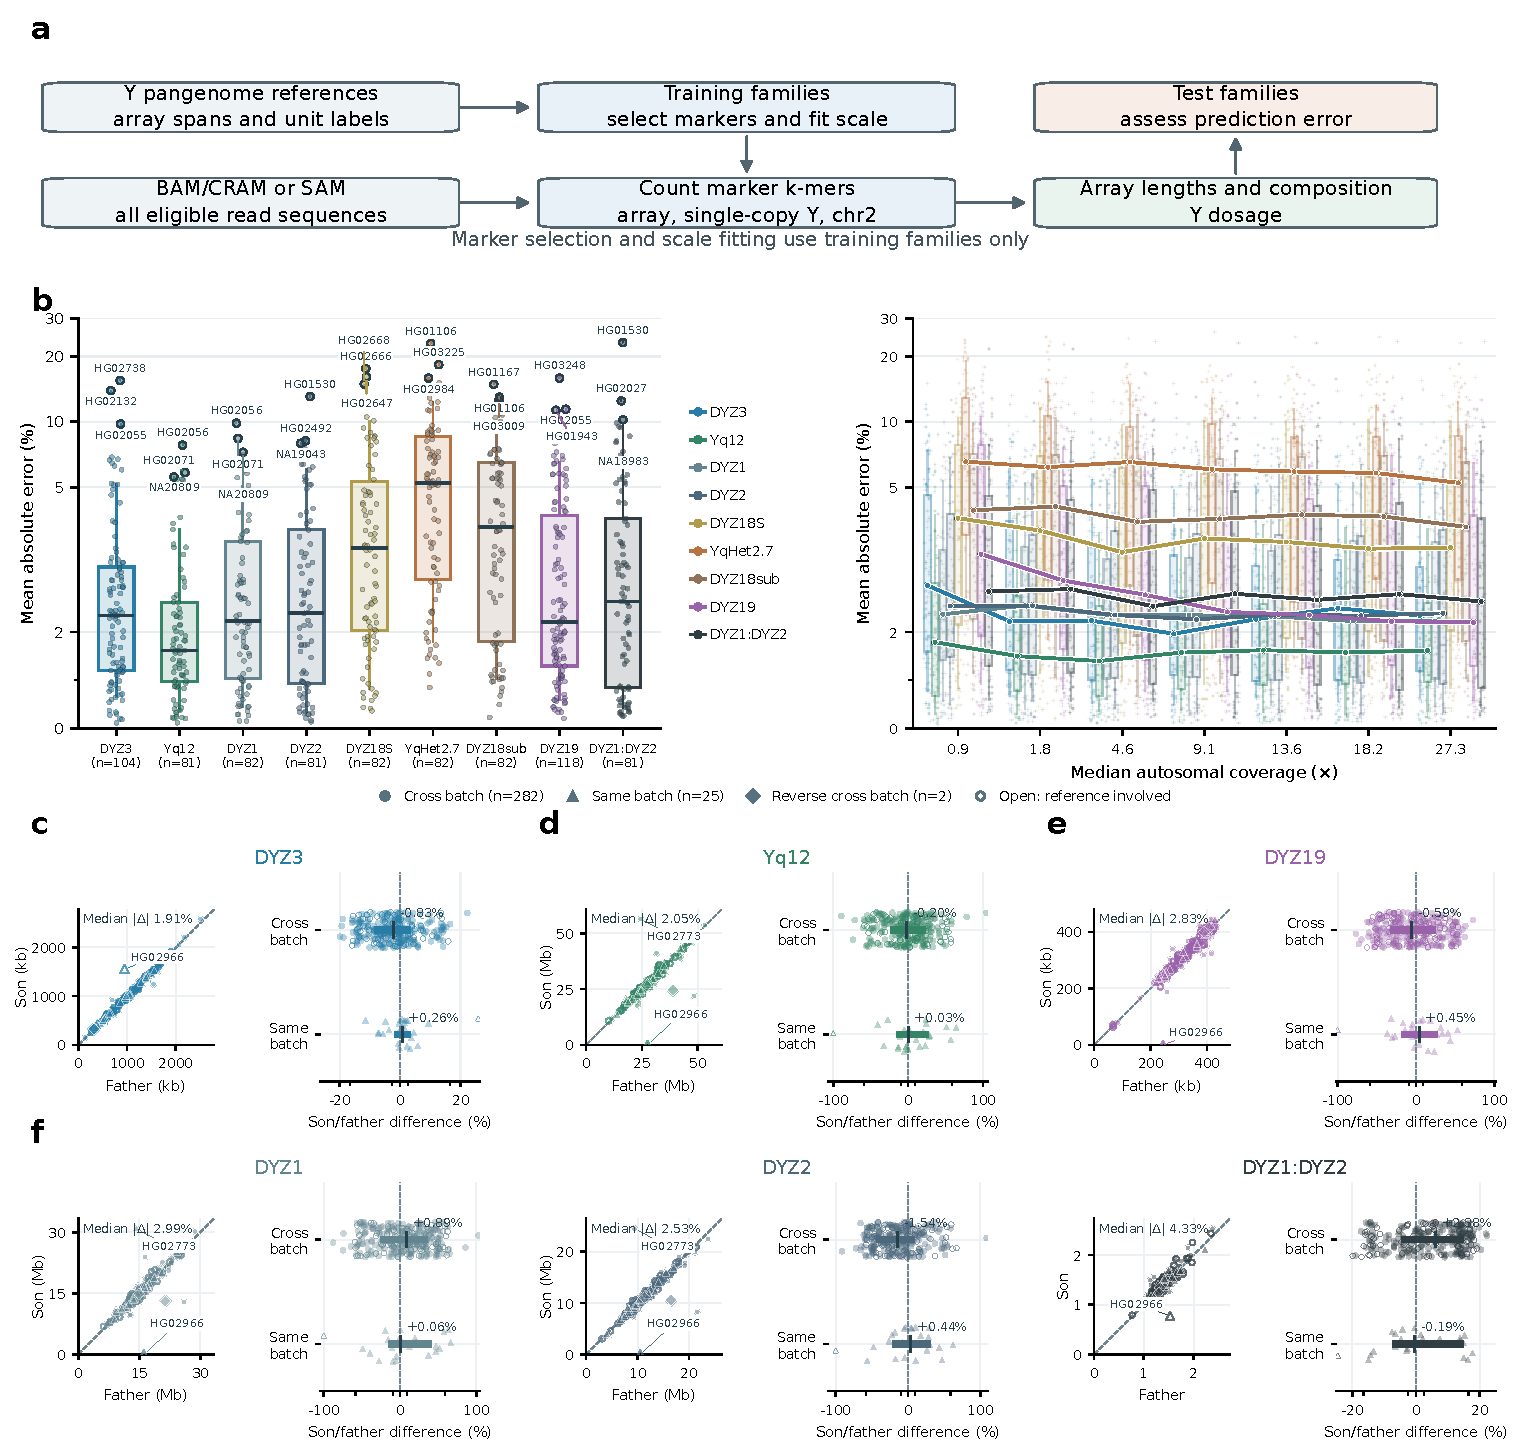
\includegraphics[width=\textwidth]{figures/figure1_draft.pdf}
\caption{\textbf{Pangenome-based calibration, prediction accuracy and pedigree agreement.} \textbf{a}, yruler workflow. \textbf{b}, Eight satellite targets and the derived DYZ1:DYZ2 ratio. Left: one point per individual and one boxplot per measurement. Points average ten absolute errors from random five-fold splits (approximately 80/20 training/test; identical FamilyIDs kept together). Ratio errors pair component predictions from the same individual and fold. Right: the same summary at seven measured median autosomal coverages; test reads are thinned and training reads retain full depth. Curves connect medians of the individual means; coverage groups are equally spaced. Boxes: 25th--75th percentiles; medians; whiskers: 10th--90th. Counts denote individuals. Labels identify the three highest individual mean errors per measurement. Error axes are linear through 5\% and logarithmic above; all points are retained. YqHet2.7 and DYZ18sub use the copy-adjusted targets. \textbf{c--e}, Father--son comparisons for DYZ3, Yq12 and DYZ19. \textbf{f}, DYZ1, DYZ2 and their length ratio, left to right. Each comparison shows estimates in all 309 pairs beside signed differences in 282 original-father/additional-son and 25 same-batch pairs. Diagonals mark equality; difference segments show interquartile ranges and medians. Open points identify 78 pairs involving a calibration reference. Shapes distinguish batch contrasts. Difference axes are logarithmic outside $\pm5\%$. Ratio axes are dimensionless. All eight targets and the ratio are shown at larger scale in Supplementary Fig.~\ref{fig:all-pedigrees}. Pedigree agreement combines measurement error and biological variation.}\label{fig:method}
\end{figure}

\subsection{Aligners, platforms and read groups}\label{sec:res-groups}
On 115 individuals with both NYGC BWA CRAMs and DRAGEN 3.7.6 BAMs, whole-file counting with the development marker set produced identical summary files. Because all eligible read sequences were counted, differences in where those reads aligned did not affect the estimates. This comparison concerns two representations of the same sequencing data; it does not test independent libraries or sequencing instruments.

For indexed DRAGEN BAMs, we also tested a reduced set of genomic regions that captures reads carrying the array and depth markers, together with unmapped reads. We chose additional windows on 30 individuals and evaluated the resulting BED on a further 100. Across the eight satellite classes in this development test, the range of the BED-to-whole normalized abundance ratio was 0.26--0.42 percentage points over all 130 individuals. Median ratios were 1.0018--1.0055, so a separate calibration is needed for this mode. With the final markers, BED and whole-file estimates of the 1,597 1kGP males with estimates differed by medians of $+0.28\%$ to $+0.48\%$ across the eight classes, with 99th percentiles of absolute differences of at most 0.75\%; the largest difference, 6.94\% for DYZ2, was in HG02966, whose Yq satellite signal is near absent. Mean processing time was 22.32 s for the restricted regions, compared with a recorded whole-file mean of 124.04 s. These are local-file measurements and do not include a cohort download.

In a separate 16-thread whole-CRAM optimization experiment on HG00126, the ten-class prototype processed the file in approximately 79--86 s, with peak resident memory of approximately 5.4--6.2 GB depending on buffering. This establishes a computational baseline rather than a final cohort-wide runtime claim.

yruler is calibrated and evaluated on Illumina whole-genome reads.

\draftnote{Repeat the alignment and restricted-region checks with the final markers and mode-specific calibration. Final runtime reporting needs a fixed software build, hardware description and separation of compute time from remote I/O. Long-read and Hi-C results require their own validated calibrations before quantitative claims are added.}

\subsection{Y dosage and sample quality}\label{sec:res-dosage}
The 40 samples recorded as female had Y dosage at most 0.0078. Of 1,599 male-labelled samples, 1,597 had estimates and two lacked estimates. Low-dose samples were retained when their estimates were available; arm-imbalanced and Yp-depleted profiles were excluded from population summaries. HG02300 is female in the corrected public metadata; negligible Y signal alone does not establish chromosome loss.

Normalizing satellite counts to single-copy Y abundance separates estimated length per Y from the amount of Y-bearing material, but cannot rescue negligible Y coverage. Dosage below 0.9 is a descriptive flag rather than an exclusion criterion. Elevated dosage also motivates inspection: HG01967 has dosage 1.3499 and DYZ19 86,383 bp and is retained as an unusual estimate for follow-up, outside population summaries. Neither low nor high dosage is assigned a cause from this ratio alone. In Fig.~\ref{fig:biology}b, satellite-length and length-ratio labels identify up to three observations per pooled 1.5-interquartile-range tail, additionally requiring at least 50\% deviation from the median of the displayed clade. HG01967 and HG02966 are also labelled in Yq12 and DYZ19 when they meet this minimum deviation; the father--son pair NA18910--NA18911 is similarly labelled in DYZ19. Dosage labels identify all observations above 1.30. These display thresholds suppress labels for small deviations in narrow distributions; they are descriptive choices, not validated biological or technical cutoffs, and do not establish measurement error or account for pedigree dependence.

\subsection{Pedigree agreement and empirical relatedness}\label{sec:res-pedigree}
The 309 father--son pairs had median absolute relative differences of 1.91\% for DYZ3 and 2.05\% for Yq12. Signed medians were $-0.64\%$ and $-0.18\%$, respectively. The 282 original-father/additional-son pairs had signed medians $-0.83\%$ and $-0.20\%$; the 25 same-batch pairs had $+0.26\%$ and $+0.03\%$. Median absolute differences were 2.83\% for DYZ19, 2.99\% for DYZ1, 2.53\% for DYZ2 and 4.33\% for the DYZ1:DYZ2 ratio (Supplementary Fig.~\ref{fig:all-pedigrees}). Seventy-eight pairs involve a reference individual. Pedigree agreement combines measurement error and biological variation; it is not independent calibration-reference accuracy.

Public KING estimates support all 307 recorded father--son relationships. Ten additional close-kinship links across different FamilyIDs occur in both reports, with two further links present in only one report. Retaining one included representative per recorded family gives 1,260 samples; using connected components of both kinship reports gives 1,273. These sensitivity subsets retain the DYZ19 separation and similar DYZ1:DYZ2 summaries (Table~\ref{tab:relatedness}).

HG01527 and HG01529 are father and son (IBS010), supported by KING kinship near 0.25 and near-zero IBS0. Their DYZ18S estimates are 592,002 and 585,224 bp and provide one familial observation. HG02965 and HG02966 are also a supported father--son pair (NG20). The reference father has Yq12 27.58 Mb and DYZ19 244.6 kb; the son has 59.9 kb and 300 bp. These values indicate marker depletion far below the calibration range; structural boundaries require sequence confirmation.

The NG20 trio comprises father HG02965, mother HG02964 and son HG02966. DYZ3 estimates are 0.951 Mb and 1.560 Mb in the father and son, with Y dosage 1.0427 and 1.2227. Multiplying $\widehat L_{ic}$ by $D_i$ cancels their shared Y denominator. The son-to-father autosomal-normalized DYZ3 signal ratio is 1.92; exact doubling would predict a son length of 1.622 Mb. Near doubling together with distal satellite depletion motivates an isodicentric Y hypothesis \cite{Lange2009}, but reuses the same marker data. Junction-spanning sequence and a separate DNA source are needed to establish chromosome structure and distinguish donor variation from cell-line change. HG01967 is father of daughter HG01969 in a different trio (mother HG01968), which supplies no paternal Y transmission comparison.

\begin{table}[tbp]
\caption{Relatedness and calibration-panel sensitivity. J-short counts J2a1a1 calls and J-other the remaining J calls; their DYZ19 ranges are separated in every subset. Ratio is the median DYZ1:DYZ2 base-pair ratio, and $\rho$ is the Spearman correlation. Representatives were selected lexicographically without using satellite measurements. KING components use the union of two public first/second-degree reports and do not establish absence of distant kinship.}\label{tab:relatedness}
\centering
\small
\begin{tabular}{lrrrrr}
\toprule
Subset & $n$ & J-short & J-other & Ratio & $\rho$ \\
\midrule
Population analysis subset & 1,587 & 42 & 44 & 1.368 & 0.824 \\
Outside reference panel & 1,451 & 37 & 40 & 1.366 & 0.825 \\
Y dosage at least 0.9 & 1,576 & 41 & 44 & 1.368 & 0.823 \\
One per recorded family & 1,260 & 37 & 37 & 1.362 & 0.835 \\
One per KING component & 1,273 & 37 & 37 & 1.362 & 0.833 \\
\botrule
\end{tabular}
\end{table}

A separate development dataset contained 305 father--son pairs: 278 main-direction cross-batch, 25 same-batch and two reverse cross-batch. Median absolute differences were 1.93\% for DYZ3 and 2.01\% for Yq12; the main-direction DYZ3 signed median was $-0.83\%$ (Supplementary Fig.~\ref{fig:development-checks}). These measurements used an earlier calibration and are retained separately from the current 309-pair analysis. No batch adjustment was applied to either display.

Transmission agreement combines technical effects and possible biological variation. The few-kilobase DYZ2 variants resolved in CEPH 1463 \cite{Porubsky2025} illustrate changes below the percent-level resolution of a typical Yq12 measurement. Neither pedigree agreement nor an apparent directional difference establishes a mutation rate.

\subsection{Array lengths in 1000 Genomes males}\label{sec:res-catalog}
All 1,597 male-labelled samples with estimates have eight satellite measurements, with 136 calibration references and 1,461 other individuals (Fig.~\ref{fig:biology}; Supplementary Fig.~\ref{fig:frozen-population}). Population summaries exclude ten arm-imbalanced or Yp-depleted samples and retain concordantly low-dose profiles with available estimates. Median lengths in the 1,587 included individuals were 858,548 bp for DYZ3, 26,977,866 bp for Yq12, 15,337,971 bp for DYZ1, 10,776,512 bp for DYZ2, 330,357 bp for DYZ19. These values describe the analysed sample, whose population representation is uneven.

DYZ3 had a median of 318,981 bp in 282 R1b individuals and 980,633 bp in the other 1,305, recovering the reported association \cite{Hallast2023}. H had the largest broad-lineage median (1.350 Mb; 71 individuals); R1a had 540,958 bp in 100 individuals. O had median Yq12 34.8 Mb. The 465 included E chromosomes had DYZ3 and DYZ19 medians of 1,091,924 and 248,275 bp, respectively.

HG04006 has the largest DYZ3 estimate in the analysed sample, 2.769 Mb, beyond the longest calibration array; independent measurement is needed. Father HG02684 and son HG02686 have DYZ3 estimates of 2.51 and 2.58 Mb, with DYZ1:DYZ2 base-pair ratios 2.38 and 2.53. Their resemblance is one familial observation.

\subsection{Population tests of compositional balance}\label{sec:res-balance}
DYZ1 and DYZ2 estimates across the 1,583 population-summary individuals are correlated (Spearman $\rho=0.8236$), with median base-pair ratio 1.3682 and first--99th percentiles 0.9621--2.0408. Family and public-kinship pruning, outside-reference-panel estimates and the earlier dosage threshold give similar ratio summaries (Table~\ref{tab:relatedness}).

The 91 assembly annotations provide a separate composition view: DYZ1 base-pair fractions range from 44.5\% to 66.8\%, and the assigned classes plus unannotated sequence partition each annotated span (Supplementary Fig.~\ref{fig:yq12-composition}). Those fractions do not directly establish equal repeat-unit counts. Balanced DYZ1:DYZ2 unit abundance and evolutionary coupling were already reported in the assembly resource \cite{Hallast2026}.

The remaining population test is whether supported departures from a declared unit-equivalent balance exceed joint annotation and measurement uncertainty and recur in independent data. It must address batch, cohort and family dependence. The present correlation or a ratio above one is insufficient to claim a novel exception, functional constraint or selection.

\subsection{Short DYZ19 arrays in sampled J2a1a1 chromosomes}\label{sec:res-lineages}
All 42 sampled J2a1a1 chromosomes had DYZ19 estimates of 61,109--77,003 bp, whereas the other 44 included J chromosomes spanned 221,264--307,059 bp. The short-state calls split between J2a1a1a (17 individuals) and J2a1a1b (25). Thirty-seven short-state individuals lie outside the calibration panel. Retaining one per documented family or public-kinship component leaves 37 short-state versus 37 other J chromosomes with the same separation.

This extends the short DYZ19 observation in HG02492 \cite{Hallast2023} to a larger sampled set. Four quality-passing J2a assembly references, HG02492, HG02735, NA20805 and NA20809, have spans of 62,421--63,669 bp, compared with a median of 321,886 bp across the 139 DYZ19 references; the J2b reference NA20905 measures 267,893 bp. Reference-panel observations and population evidence are reported separately.

NA18910 and NA18911, a father--son pair from the YRI cohort (E1a2a1b2), also have short DYZ19 estimates of 85,090 and 79,254 bp, with Y dosage 1.0471 and 1.0461. Public KING reports support their relationship. They provide one familial observation outside J2a1a1; the current sample contains no other E1a2a1b2 individuals. Measurements in separate sequencing batches do not establish a short state throughout that lineage.

The provisional SNP tree recovers a clade containing all 42 J2a1a1 chromosomes; J2a1a2 lies outside that clade (Supplementary Fig.~\ref{fig:j-dyz19}). This supports a lineage-associated short-array state in the sampled J2a1a1 chromosomes. The separate short-state YRI family and remaining fine-scale classification discordances require additional checks before inferring origins or transitions. The current tree is not time-calibrated.

\begin{figure}[tbp]
\centering
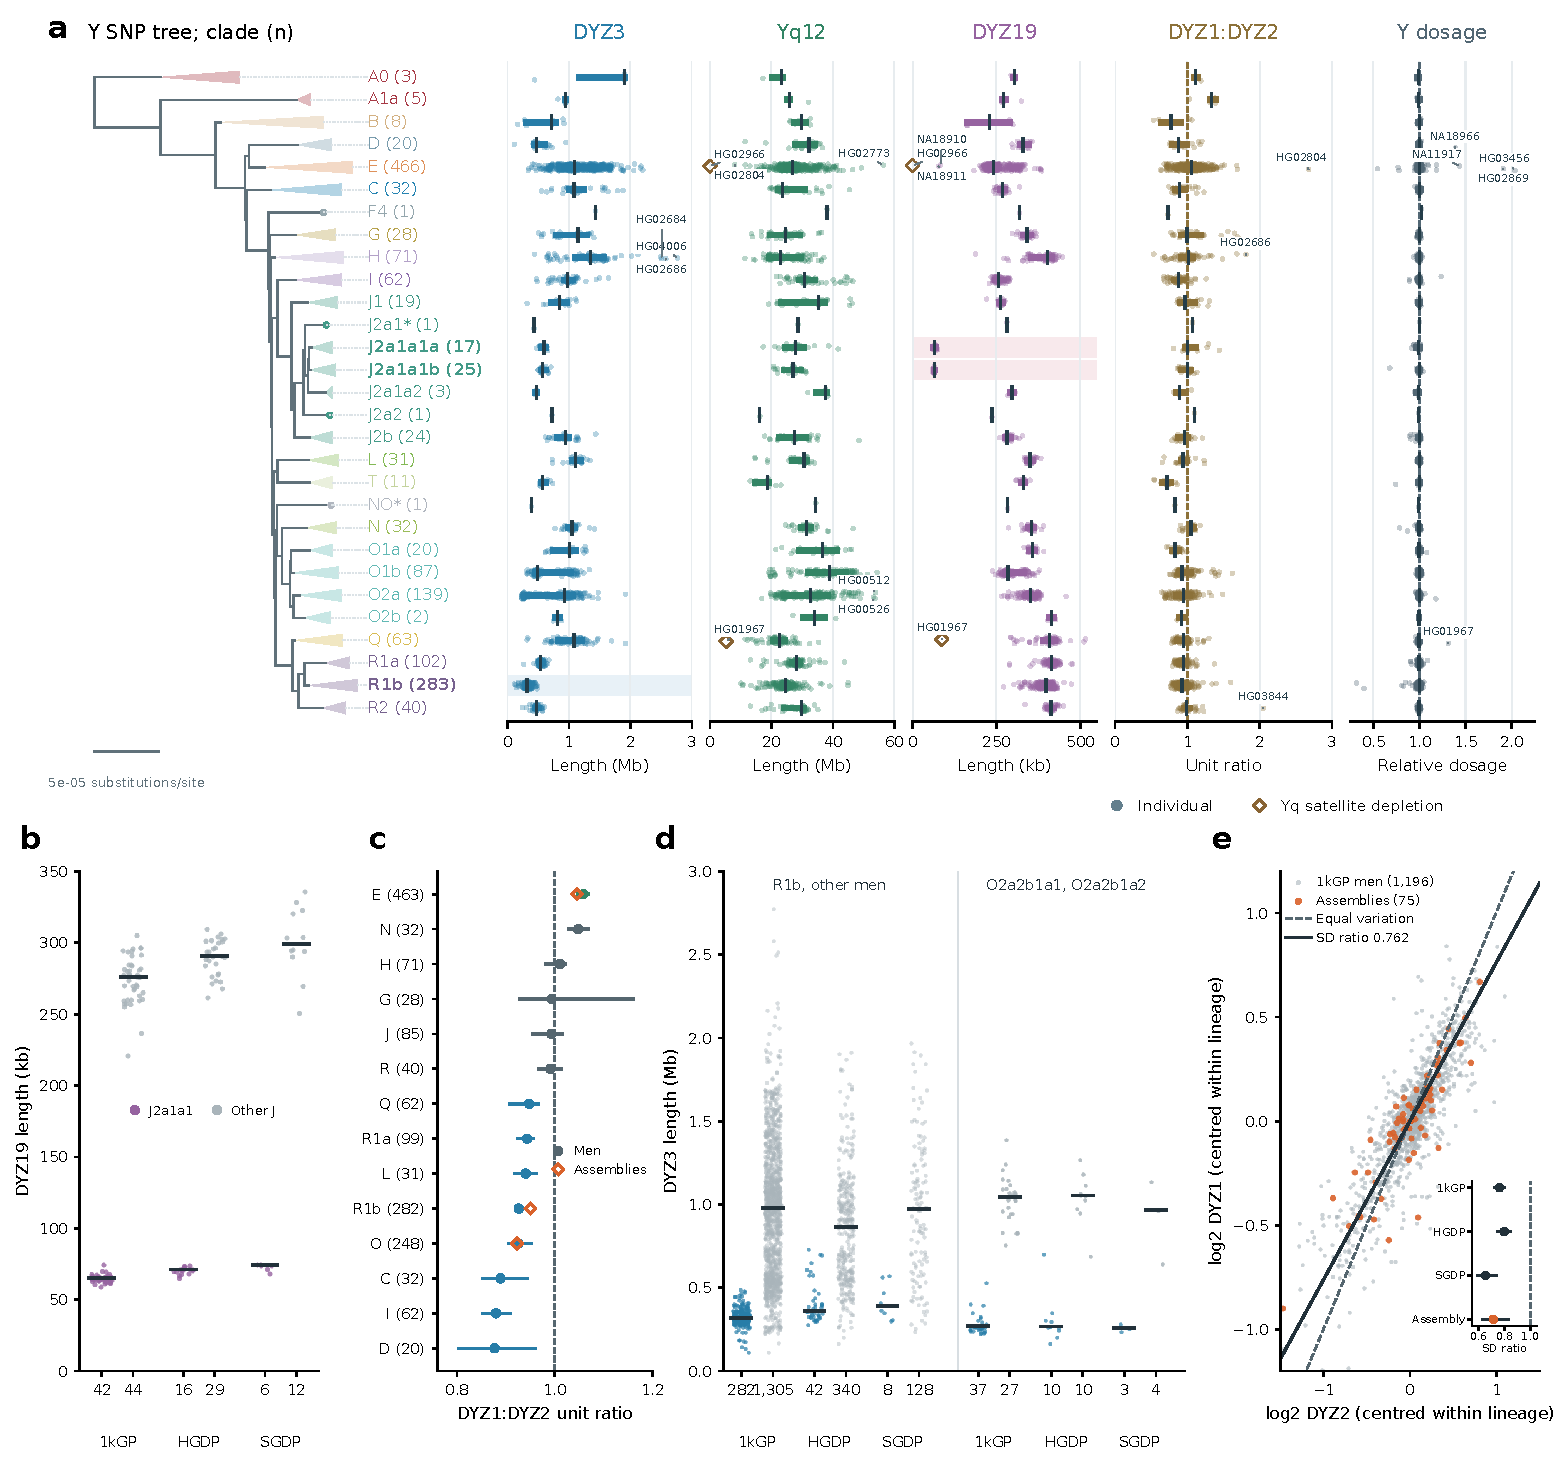
\includegraphics[width=\textwidth]{figures/figure2_draft.pdf}
\caption{\textbf{Y satellite variation across paternal lineages.} \textbf{a}, Geographic coverage of 1,597 1kGP individuals with estimates and HGDP/SGDP cohort manifests: 2,302 unique individuals after deduplication. Coordinates are cohort-reported population locations. Pie area scales with sample counts; sectors and legend counts show paternal Y lineages. Grey denotes two pending assignments; seven SGDP records reported as female and one additional record without Y signal are excluded (Online Methods). \textbf{b}, SNP tree aligned to DYZ3, Yq12, DYZ19, the DYZ1:DYZ2 length ratio and Y dosage in 1,597 males, including 136 calibration references whose estimates are not independent validation. Dashed line: dosage 1. Homogeneous clades are collapsed; triangles retain within-clade branch-length extent. Stars mark unresolved calls. Diamonds identify reduced Yq satellite signal in HG01967 and near-absent signal in HG02966, only in Yq12 and DYZ19. HG02966 is the son of reference HG02965, whose satellite estimates are within the usual range. All four arm-imbalanced and six Yp-depleted profiles remain visible and are excluded from summaries. Labels identify substantial satellite deviations and dosage above 1.30 (Online Methods). Lines: interquartile ranges; marks: medians among 1,587 included individuals. Background highlights R1b--DYZ3 and J2a1a1--DYZ19. The provisional tree uses the callable-region SNP analysis with full search and branch-support calculations (Online Methods).}\label{fig:biology}
\end{figure}
\clearpage

\section{Discussion}\label{sec:discussion}
The Y pangenome makes satellite variation accessible as assembled sequence across individuals, but an assembly for every sequenced genome remains impractical. yruler uses complete arrays from this pangenome to define measurement targets and select markers, then estimates array length directly from sequencing-read abundance. The implementation measures total DYZ3 and Yq12 abundance alongside satellite sequence components. Measuring several targets in the same pass also exposes differences among arrays that would be obscured by a single estimate of Y heterochromatin content. The pangenome supplies sequence diversity and calibrated references. Grouped cross-validation assesses prediction within the current reference collection; lineage exclusion tests transfer to represented broad groups; performance in independent cohorts remains to be established.

The main contribution is the combination of multi-array measurement, explicit assembly calibration, independent evaluation and Y dosage. Earlier studies already measured DYZ3 or DYZ1 from short reads \cite{Miga2014,Altemose2014}, and DYZ1 coverage has been studied in more than one thousand males \cite{SanRoman2024}. An empirical comparison must therefore assess accuracy and generalization on shared individuals, while acknowledging differences in sequencing depth and library preparation. Comparisons of previously published estimates with contemporary reads are not controlled comparisons of algorithms alone. Likewise, selecting a similar centromere reference haplotype \cite{Shiraishi2026} addresses a different target from directly measuring its length.

Our reference annotation emphasizes that an array does not have a unique length until its boundaries and sequence classes have been specified. A reference active HOR array, a broader alpha-satellite interval and the bases matching an HOR profile are different targets. Yq12 span and DYZ1-plus-DYZ2 unit bases also differ because the region contains smaller satellite classes and intervening sequence. Clear target definitions are needed both for calibration and for biological comparisons. Even quality-passing assemblies remain measurements with possible annotation and assembly errors; the reference checks reduce this uncertainty without eliminating it.

The smaller arrays require separate evaluation. Closely related repeat classes may share most candidate markers, leaving a small or biased set of diagnostic sequences. An aggregate result for Yq12 does not establish the accuracy of every component. Each output must be judged against its reference variability, held-out prediction error and relevant short or depleted states before it is used to infer population variation.

Sequencing protocol is a second limit. Counting all eligible read sequences removes dependence on their alignment positions for the matched files tested here, but it cannot restore sequence that a library or instrument underrepresents. Platform-specific scale factors correct average shifts, not arbitrary library-specific distortions. Restricted-region counting adds another condition: its calibration and capture efficiency depend on the alignment pipeline. These effects require validation at the level of the read group and analysis mode used in a cohort.

Pedigrees illustrate how measurement bias can affect a biological interpretation. A small directional father--son difference can arise when generations fall in different sequencing batches. Correcting such differences also requires care: using the same relatives to fit a batch adjustment and to test a transmission effect would couple calibration to the outcome. Independent calibration, explicit batch contrasts and family-aware uncertainty are needed before assigning a directional change to satellite biology. At the present percent-level resolution, pedigree concordance is most useful for detecting inconsistency; it does not measure the rate of small repeat-unit mutations.

The biological opportunity is to test the extent and exceptions of satellite compositional balance and to map supported array states across populations. Balanced DYZ1:DYZ2 abundance and their evolutionary coupling are already documented in the assembly resource \cite{Hallast2026}. A larger read-based catalog can examine reproducible departures, their distribution within lineages and their persistence across cohorts. The preliminary DYZ19 separation extends beyond the calibration panel and survives close-kinship pruning, motivating replication of the short state within fine J sublineages and neighbouring groups.

These comparisons require a distinction between reference-panel observations and independent population evidence. The SNP tree supplies branch lengths for a provisional phylogenetic display; fine-scale topology and prediction uncertainty still limit state-transition inference. The tree has no time calibration. Measurement covariance, pedigree dependence and cohort effects must accompany models of satellite dynamics. A fitted tendency towards a common composition would not by itself demonstrate functional constraint or selection. Y dosage provides a parallel quality measurement for interpreting unusual array estimates.

\draftnote{Revise this discussion after expanding the population analysis, unit-equivalent composition analysis and external evaluation. Add calibrated interval coverage and a same-data comparison with published measurements where the measurement targets are comparable.}



\section{Conclusions}\label{sec:conclusions}
yruler uses the Y pangenome to measure satellite array lengths, repeat composition and Y dosage from sequencing reads. It combines targets for DYZ3, total Yq12 and satellite sequence components in one counting framework. Grouped cross-validation establishes internal performance for eight outputs, and preliminary population profiling identifies consistently short DYZ19 estimates within the sampled J2a1a1 calls. External validation and independent structural confirmation will define the final scope. These measurements extend the study of inherited Y satellite variation from complete arrays in the pangenome to existing genome collections.

\section{Methods}\label{sec:methods}

\subsection{Reference arrays}\label{sec:m-truth}
Reference lengths were taken from the 142-individual Y assembly resource \cite{Hallast2026}. HPRC release 2 assemblies \cite{HPRCRelease2} supplied an array only when the corresponding array in the primary resource did not pass the completeness criteria. A retained array had to lie on one contig, with at least 100 kb of flanking sequence on both sides and no assembly gap. We excluded an array if any overlapping 1 kb window was flagged as erroneous by all four combinations of Flagger or NucFlag with HiFi or ONT reads. An array without the required quality evidence was not treated as quality-passing. This rule tests concordant evidence of assembly error; it does not imply that every retained base is correct.

Reference eligibility was assessed separately for each array: inclusion of a genome in a pangenome resource, or a favourable genome-wide assembly metric, did not establish completeness of its DYZ3, Yq12 or DYZ19 sequence. Passing one target did not imply eligibility for another. The HPRC2 report likewise identifies repetitive Yq as a persistent assembly limitation \cite{Lucas2026}. Inspection of the retained reference regions found no reported Hallast gap/error labels and no N bases in the 17 replacement DYZ3/Yq12 spans. Absence of gaps does not exclude collapsed or duplicated sequence. Local flags from a single quality assessment were retained for targeted follow-up; the initial inventory is retained in the development supplement.

The initial reference inventory comprised 120 DYZ3 arrays from the primary resource and nine HPRC replacements, 83 Yq12 regions from the primary resource and eight replacements, and 139 quality-passing DYZ19 main arrays. NA18879 and HG00329 were absent from the DYZ3 inventory because parts of their arrays lay on unplaced contigs. The four-track quality rule excludes the Yq12 region of HG01261 and with it its DYZ2 target, leaving 129 DYZ3, 90 Yq12 and 139 DYZ19 targets; the DYZ1, DYZ18S, YqHet2.7 and DYZ18sub targets of HG01261 are retained. The reported CV is conditional on this reference set. Independent sequence confirmation and external evaluation remain necessary.

\draftnote{Supply an accession and coordinate manifest, assembly and quality-call versions, and all per-array inclusion reasons. Verify implementation of the stated quality rule for each source. Cite the release 2 resource directly; the release 1 pangenome paper is not a substitute for this data version.}

\subsection{Satellite annotation}\label{sec:m-units}
We built profile HMMs for DYZ1, DYZ2, DYZ18, related 3.1 kb and 2.7 kb units, DYZ19 and the DYZ3 HOR. Seed searches identified full-length units, which were oriented consistently. Up to ten units per assembly and class were aligned with MAFFT 7.526 \cite{Katoh2013}, and profiles were built with hmmbuild from HMMER 3.4 \cite{Eddy2011}. DYZ3 HOR units were extracted from one HOR start to the next within the reference active-array region. The resulting profiles define assembly annotations; their role is distinct from the read-marker sets rebuilt in validation splits.

All class profiles were searched against each assembly with nhmmer \cite{Wheeler2013}. Hits were retained at an E-value of at most $10^{-10}$, with a threshold of $10^{-5}$ for DYZ19. Overlapping sequence segments were assigned to the highest-scoring model. Candidate Yq12 blocks were formed by joining segments from hits covering at least half the model across gaps of at most 100 kb, and the block with the greatest assigned support defined the annotation-derived Yq12 boundaries. Within those boundaries, DYZ1 and DYZ2 lengths were the totals of their assigned bases. For DYZ18 and the 3.1 kb and 2.7 kb classes, we joined assigned segments across gaps of at most 5 kb and retained the cluster with the greatest assigned-base total. Remaining bases within the Yq12 boundaries were labelled unassigned. DYZ18S was the sum of the DYZ18 and 3.1 kb assigned bases. DYZ18sub combines those bases with the 2.7 kb class, so it overlaps the DYZ18S and YqHet2.7 targets and is not an additional component of a partition. The main DYZ19 array was selected by the same 5 kb clustering rule; its outer coordinates defined the span used in calibration.

\draftnote{Record the seed accessions, final profile files, sampling seed and exact numbers of units. The DYZ1 seed provenance needs confirmation. Retain the distinction between the cluster's assigned-base total and its outer-coordinate span in all released tables.}

For YqHet2.7 and DYZ18sub, calibration uses a copy-adjusted target $L_i^*=L_i(c_{i,\mathrm{in}}+c_{i,\mathrm{out}})/c_{i,\mathrm{in}}$, where $L_i$ is the original annotation-derived length and $c_{i,\mathrm{in}}$ and $c_{i,\mathrm{out}}$ are assembly marker-copy counts inside and outside the original target. The adjustment is an assembly-derived marker-equivalent target, not a newly annotated physical array span. Its CV error measures agreement with that target; reductions relative to the original annotation-based benchmark cannot be interpreted solely as improved physical-length accuracy.

\subsection{Markers from the Y pangenome}\label{sec:m-markers}
Canonical 31-mers were counted in the training assembly regions with KMC 3.2.4 \cite{Kokot2017}. The common rule for satellite classes selects k-mers present in at least a fraction $p$ of eligible training assemblies, excludes k-mers found in CHM13 outside chromosome Y \cite{Nurk2022} or in at least 50\% of 99 quality-selected HPRC non-Y haplotypes, and keeps only k-mers that occur on the training Y chromosomes outside the target regions in fewer than a fraction $o$ of training assemblies. Candidate thresholds are $p$ from 0.50 to 0.95 and $o\in\{0,0.05,0.1,0.25\}$, where $o=0$ means no training assembly. DYZ18S uses the union of the DYZ18 and 3.1 kb regions. The single-copy Y denominator consists of X-degenerate-region k-mers present in at least 90\% of the training assemblies, and chromosome 2 depth markers come from a single-copy interval near GRCh38 chr2:50.0--60.0 Mb. Marker counts and coordinates are model-specific.

Within each outer training partition, $p$ and $o$ are selected per class by the leave-one-out error of the scale fit on the training individuals only. This is an internal selection criterion: its errors are not reported as the benchmark. Candidates come from a pool of k-mers present in at least 25\% of the class assemblies; for every class, split and threshold we verified that this pool contains every k-mer the training-fold rule can select. The fitted model applies the same procedure to all eligible reference individuals: markers, thresholds and $K_c$ are fitted on the full reference set, and cross-validation estimates the accuracy of this procedure. Masked superstrings \cite{Sladky2023} with zstd compression provide a compact representation without changing marker membership.

Alternative denominators and non-Y filters were compared during development. The current procedure uses the single-copy Y denominator at 90\% assembly presence and the CHM13 plus quality-selected HPRC filter. DYZ2 and YqHet2.7 markers must also contain at least 16 and 8 G or C bases of 31 (G+C content at least 51.6\% and 25.8\%), because reads poor in G+C are underrepresented in some libraries. Each floor was chosen once from 4 to 17 bases on the same males sequenced in two projects or in other Illumina runs, by leave-one-out, provided that the cross-validation median and maximum errors rose by at most 0.10 and 1.0 percentage points; the other classes have no floor. Yq12 is estimated as the Yq12 marker estimate minus its DYZ2 part (DYZ2 markers without the floor) plus the DYZ2 estimate with the floor, and cross-validation evaluates this combination. Marker counts are 6,687 for DYZ3, 672,509 for Yq12, 188,594 for DYZ1, 18,552 for DYZ2 (173,793 without the floor), 31,660 for DYZ18S, 10,345 for YqHet2.7, 30,391 for DYZ18sub and 83,972 for DYZ19, with 6,913,866 single-copy Y markers. The G+C correction curve applies to all classes.


\subsection{Read-based marker counting}\label{sec:m-counting}
yruler reads BAM and CRAM through rust-htslib and HTSlib \cite{Bonfield2021}, using the index for parallel genomic shards. Whole-file shards are 10 Mb windows plus unmapped reads; restricted-region mode uses merged BED intervals plus unmapped reads. Overlapping retrievals are deduplicated by their shard ownership so that an eligible record is counted once. Secondary and supplementary records are excluded. Primary records are retained without a mapping-quality threshold; duplicate flags are recorded in the spatial summaries but do not exclude reads from marker counting. Paired-end reads contribute as separate sequencing records, and every canonical 31-mer occurrence contributes to its marker count. Ambiguous bases interrupt k-mer generation. The current counting path does not apply a base-quality threshold.

An open-addressing hash table verifies marker membership after a Bloom filter, with thread-local caches reducing repeated lookups. A marker may contribute to multiple classes, as required when a component is also part of Yq12. Outputs include per-marker counts, class summaries, counts grouped by genomic position and normalized length estimates. SAM input is read sequentially and processed in parallel. The restricted-region BED is specific to the alignment pipeline and requires its own scale calibration.

\subsection{Length estimation}\label{sec:m-length}
For individual $i$ and class $c$, let $C_{ik}$ be the count of marker $k$ and $g(k)$ its number of G or C bases. We estimate a relative depth curve $r_i(g)$ from single-copy Y markers. Counts above 10 times the mean count plus 10 are left out as repeated sequence; the baseline is the mean of the remaining counts, and each G+C-bin mean uses the remaining counts of its markers. A bin requires at least 1,000 markers and 10,000 counts, and missing bins use the nearest supported G+C bin. The same rule applies at every sequencing depth. Dividing bin means by the baseline gives $r_i(g)$. A factor $f_i$ is the mean of $r_i(g(k))$ over the single-copy Y markers, so that
\begin{equation}
 S^{\mathrm{GC}}_{ic}=f_i\sum_{k\in M_c}\frac{C_{ik}}{r_i(g(k))},
 \qquad S_{iY}=\sum_{k\in M_Y}C_{ik}.
\end{equation}
The curve requires at least 1,000,000 single-copy Y counts; HG00126 has 117,080,371 at full depth and 3,921,538 when thinned to a fraction of 0.033. With fewer counts, yruler reports a warning and uses uncorrected sums, whereas the 1kGP analysis withholds the estimate (Y dosage, below). Single-copy Y and chromosome 2 sums are not G+C-corrected by this procedure.

The estimated length and training scale are
\begin{equation}
 \widehat L_{ic}=K_c z_{ic},\qquad
 z_{ic}=\frac{S^{\mathrm{GC}}_{ic}}{S_{iY}},\qquad
 K_c=\frac{\sum_{i\in\mathcal T_c}L_{ic}}
 {\sum_{i\in\mathcal T_c}z_{ic}},
\end{equation}
where $\mathcal T_c$ contains training individuals with an eligible reference length for class $c$. Thus, $K_c$ calibrates marker abundance to the stated reference target rather than equating marker counts to physical sequence coverage. Technology-specific models require a separate fitted $K_c$; the presence of a technology option does not by itself validate that model.

\subsection{Y dosage}\label{sec:m-dosage}
Y dosage is
\begin{equation}
 D_i=2\,\frac{S_{iY}/n_Y}{S_{i2}/n_2},
\end{equation}
where $S_{i2}$ is the raw chromosome 2 marker sum and $n_Y$ and $n_2$ are the marker-set sizes for the fitted model. Under balanced sequencing and one Y chromosome per diploid cell, $D_i$ is expected to be near one. Chromosome 2 copy-number changes and differential sequence representation can change this ratio. In a structurally altered Y chromosome, gains and losses of ruler-bearing regions can also change dosage; it cannot then be interpreted directly as the number of Y chromosomes or centromeres. An estimable positive length for all eight targets is required. The estimation pipeline withholds lengths when the single-copy Y markers have fewer than 1,000,000 counts, too few for the G+C curve. A uniform change in Y abundance cancels in the array-to-Y ratio, so dosage below 0.9 alone is retained as a descriptive flag. Arm imbalance is assessed separately using the chromosome-arm profiles below.


\subsection{Accuracy evaluation}\label{sec:m-benchmark}
Prediction accuracy was evaluated with ten repeats of random five-fold cross-validation, with approximately 80\% of individuals used for training and 20\% for testing in each fold. Splits were randomized subject to keeping individuals with the same recorded pedigree FamilyID in the same fold; individuals absent from the pedigree were treated as separate groups. Among the 118 unique evaluated individuals, there were 117 such groups: only HG02666 and HG02668 shared a FamilyID (GB40). Their recorded test-fold assignments agreed in all ten repeats. In each repeat, group identifiers were randomly permuted and assigned cyclically to five folds; each fold served once as the test set. Thus, train/test proportions could vary slightly with group size and target-specific reference availability. Markers, the selection of their presence and outside thresholds and $K_c$ were fitted using only the outer training folds; the G+C floors, the reference-quality rule and the target definitions were fixed before cross-validation, and each individual's error was recorded in its outer test fold. Candidate k-mer pools were checked to contain every marker that could satisfy the training-fold selection rules, including those contributed by eligible reference assemblies without read data.

We additionally excluded each of 18 broad Y lineages in turn, removing its eligible references and any recorded family shared with test individuals from training. Markers, thresholds and calibration were refitted on the remaining references. Each evaluated individual therefore has one excluded-lineage prediction per target, rather than ten repeated CV predictions (Supplementary Fig.~\ref{fig:lineage-validation}). The same target-specific individuals were evaluated in both analyses.

For sequencing-depth sensitivity, test reads were thinned to fractions 0.667, 0.5, 0.333, 0.167, 0.067 and 0.033; training reads remained at full depth. All ten repeats and five folds were retained at every fraction, with the same test assignments as full-depth CV. Each fraction contains 7,120 predictions across the eight targets. All 7,120 full-depth predictions match the main CV in sample, repeat, fold and error. Coverage was measured from chromosome 2 marker counts in each thinned run; group coordinates are medians across the 118 unique evaluated individuals, each counted once. The seven median coverages span 0.90--27.25$\times$.

Absolute relative error is $100|\widehat L_i/L_i-1|$, and signed relative error is $100(\widehat L_i/L_i-1)$. Figure~\ref{fig:method}b gives each individual equal weight: each point is the arithmetic mean of ten absolute out-of-fold percentage errors, one per repeat. Errors are made absolute before averaging. Boxes span the 25th--75th percentiles, central lines show medians and whiskers end at the 10th and 90th percentiles; all individual points remain visible. Labels identify the three highest individual mean errors per target, with ties resolved by sample identifier. In the coverage panel, each point likewise averages ten absolute errors for one individual at one depth fraction. Curves connect the medians of these individual means. Boxes at different coverages are equally spaced and labelled by measured median autosomal coverage, rather than by the thinning fraction. Error axes are linear through 5\% and logarithmic above. Supplementary Fig.~\ref{fig:cv-folds} retains every test-fold distribution. Table~\ref{tab:accuracy} reports the mean of ten repeat-specific median errors, which differs from the median of the displayed individual means; maxima refer to single out-of-fold predictions. Repeated predictions are not independent biological individuals.

The DYZ1:DYZ2 length ratio is a derived, dimensionless measurement rather than an additional satellite class. Its validation pairs the two component predictions for the same individual, repeat and test fold; fold assignments were checked to match. Ratio error is $100| (\widehat L_{\mathrm{DYZ1}}/\widehat L_{\mathrm{DYZ2}})/(L_{\mathrm{DYZ1}}/L_{\mathrm{DYZ2}})-1|$, calculated before summarizing. The paired set contains the 81 individuals with both references, with 810 full-depth predictions and ten repeats at each reduced coverage. Each excluded-lineage ratio likewise uses the two component predictions from the same held-out lineage. The ratio has no separately fitted calibration or marker set.

The historical Miga/Altemose samples \cite{Miga2014,Altemose2014} informed method development. Their median errors were 2.85\% for DYZ3 (20 individuals), 1.16\% for Yq12 (12) and 2.72\% for DYZ19 (21). These comparisons are treated as development evidence. The accuracy assessment reported here uses cross-validation; a separate cohort that did not inform method design is needed to evaluate external performance. We report point estimates without calibrated prediction intervals.

\subsection{Pedigrees and sequencing batches}\label{sec:m-pedigree}
Father--son relationships were taken from the recorded 1000 Genomes parents; CEPH 1463 development comparisons used the published pedigree \cite{Porubsky2025}. Intersecting documented pairs with the 1,597 male-labelled samples with estimates gave 309 father--son pairs: 282 have fathers in the original 2,504-sample batch and sons in the additional 698-sample batch, 25 have both in the additional batch, and two have the opposite cross-batch direction (NA07034--NA07048 and NA12056--NA10851). All 309 pairs are retained in the absolute-length panels and overall summaries. The main signed-difference panels summarize the 282 original-father/additional-son pairs and the 25 same-batch pairs; the two reverse-direction pairs are shown separately in the absolute-length panels. Seventy-eight pairs involve at least one calibration-reference individual; the other 231 involve two individuals outside that panel. Arm-flagged pairs remain visible for structural follow-up.

All eight satellite targets and the DYZ1:DYZ2 ratio are compared in Supplementary Fig.~\ref{fig:all-pedigrees}. Its signed-difference panels additionally retain the two reverse-direction pairs as a separate group. Signed differences are $100(\widehat L_{\mathrm{son}}/\widehat L_{\mathrm{father}}-1)$, with absolute values used for concordance. Absolute-length axes have matching limits and a diagonal denoting equality. Shapes distinguish batch contrasts, including the reverse direction in the absolute-length panels, and open points mark pairs involving a calibration reference. The largest labelled differences give son identifiers. All pairs contribute to overall concordance; the two reverse-direction pairs are not pooled into the signed-difference summaries of the main cross-batch direction. Signed-difference axes are linear within $\pm5\%$ and logarithmic outside; summary lines show medians and interquartile ranges. No batch adjustment was applied. Pedigree agreement combines measurement differences and potential biological variation and is not a mutation-rate estimate.

Close relatedness was assessed using two public GRCh38 KING-robust first/second-degree pair reports for the 3,202-person 1kGP collection from \url{https://www.cog-genomics.org/plink/2.0/resources} (retrieved 27 October 2026). Published estimates were joined to sample and pedigree records by exact identifiers, retaining both reported coefficients and IBS0 values. Both reports support all 309 father--son pairs. Among the 118 unique CV individuals, 115 are covered by the corrected public metadata; neither report adds a cross-FamilyID first/second-degree link among those covered individuals. The remaining three are outside this resource. Ten pairs across different FamilyIDs occur in both reports, including one with kinship approximately 0.264; two further pairs occur only in the first report. Their exact pedigree relationships were not assigned.

Sensitivity analyses retain the lexicographically first sample within each recorded family (1,260 representatives) or within each connected component of the union of the two reported kinship graphs (1,273 representatives). Selection does not use satellite measurements. The component rule is conservative and is not a maximum independent-set calculation. The reports are thresholded at first/second degree, so absence of a reported pair does not establish absence of more distant relatedness.

All 1,639 samples were also covered by the resource's corrected sex metadata. HG02300 is coded male in the source pedigree but female in the corrected metadata. Its missing Y estimate is therefore reported with this metadata discrepancy. Source codes are retained for sample accounting; low Y signal alone is not assigned a biological cause.

\subsection{Population descriptors and reference-panel representation}\label{sec:m-descriptors}
Y haplogroups describe branches of the paternal genealogy inferred from Y-linked variants. They provide the grouping relevant to these Y satellite measurements and do not describe an individual's genome-wide ancestry, ethnicity or identity. Collapsing branches for display does not imply uniform satellite lengths within a lineage. The 1kGP population and superpopulation labels are retained as source metadata for sample accounting; they were not used to select markers, fit calibration scales or assign random cross-validation folds. Geographic coordinates describe locations reported by the source cohorts. We did not estimate genome-wide ancestry from Y haplogroups or geographic labels.

We tabulated representation by target and Y lineage using the array-reference manifests, unique individuals in the ten-repeat CV predictions and the analysed cohort (Table~\ref{tab:reference-lineages}). Reference eligibility and read-based evaluation are counted separately; repeated predictions count once. Yq12 and its five component outputs share the reference and evaluated-individual sets. Grouping follows the archived ISOGG classification hierarchy, independently of the exploratory SNP-tree topology. Ten unique reference individuals lack calls in this lookup and remain unassigned; they are distinct from the two pending HGDP/SGDP calls in the geographic map. No call was inferred from a population label.

Representation is uneven at the displayed resolution. Among assigned references, O1a has a DYZ3 and DYZ19 reference but no Yq12 reference; O2b and several fine J groups have none for the three array targets. These counts identify limitations of the available panel, not the fraction of genetic diversity captured. Unassigned references limit statements about absent lineages. Leave-one-lineage-out evaluation tests prediction after excluding represented broad groups; it does not establish accuracy in every sparsely represented or unsampled subclade.

\begin{table}[p]
\caption{Y-lineage representation of the reference panels and analysed cohort. Each target column gives eligible assembly references / individuals evaluated in cross-validation. The Yq12 column also describes DYZ2; DYZ1, DYZ18S, YqHet2.7 and DYZ18sub add HG01261 (lineage R1b), whose Yq12 and DYZ2 lengths are excluded by the assembly-quality rule. Counts use the archived ISOGG 2019 classification hierarchy, independently of the inferred SNP tree. Unassigned denotes missing calls in the archived lookup, not a biological lineage. Reference individuals can also occur in the cohort; columns are not disjoint. A nonzero count does not establish adequate coverage of a lineage, and zero does not establish absence of a related reference in an ancestral or neighbouring clade.}\label{tab:reference-lineages}
\centering\small
\begin{tabular}{lrrrr}
\toprule
Y lineage & Cohort & DYZ3 & Yq12 & DYZ19 \\
\midrule
A0 & 3 & 1 / 1 & 1 / 1 & 2 / 2 \\
A1a & 5 & 3 / 3 & 3 / 3 & 3 / 3 \\
B & 8 & 3 / 3 & 2 / 2 & 3 / 3 \\
D & 20 & 5 / 2 & 1 / 1 & 2 / 2 \\
E & 466 & 24 / 20 & 16 / 16 & 32 / 27 \\
C & 32 & 3 / 1 & 2 / 1 & 6 / 3 \\
F4 & 1 & 1 / 1 & 1 / 1 & 1 / 1 \\
G & 28 & 3 / 3 & 3 / 3 & 4 / 4 \\
H & 71 & 4 / 3 & 2 / 2 & 4 / 3 \\
I & 62 & 4 / 3 & 3 / 2 & 3 / 3 \\
J1 & 19 & 3 / 3 & 2 / 2 & 3 / 3 \\
J2a1* & 1 & 0 / 0 & 0 / 0 & 0 / 0 \\
J2a1a1a & 17 & 2 / 1 & 1 / 1 & 1 / 1 \\
J2a1a1b & 25 & 3 / 2 & 3 / 2 & 3 / 2 \\
J2a1a2 & 3 & 0 / 0 & 0 / 0 & 0 / 0 \\
J2a2 & 1 & 0 / 0 & 0 / 0 & 0 / 0 \\
J2b & 24 & 1 / 1 & 1 / 1 & 1 / 1 \\
L & 31 & 1 / 1 & 1 / 1 & 2 / 2 \\
T & 11 & 2 / 2 & 1 / 1 & 2 / 2 \\
NO* & 1 & 1 / 1 & 0 / 0 & 1 / 1 \\
N & 32 & 5 / 5 & 5 / 5 & 6 / 6 \\
O1a & 20 & 1 / 1 & 0 / 0 & 1 / 1 \\
O1b & 87 & 4 / 4 & 2 / 2 & 4 / 4 \\
O2a & 139 & 14 / 13 & 11 / 11 & 14 / 14 \\
O2b & 2 & 0 / 0 & 0 / 0 & 0 / 0 \\
Q & 63 & 6 / 6 & 4 / 4 & 6 / 6 \\
R1a & 102 & 7 / 5 & 5 / 5 & 7 / 5 \\
R1b & 283 & 15 / 15 & 12 / 12 & 15 / 15 \\
R2 & 40 & 3 / 1 & 1 / 1 & 3 / 1 \\
Unassigned & 0 & 10 / 3 & 7 / 1 & 10 / 3 \\
\midrule
Total & 1597 & 129 / 104 & 90 / 81 & 139 / 118 \\
\botrule
\end{tabular}
\end{table}


\subsection{Population summaries and composition}\label{sec:m-population}
We analysed 1,639 1000 Genomes samples using the procedure calibrated on all eligible reference individuals. Of 1,599 samples recorded as male, 1,597 had estimable positive lengths for all eight targets; twelve had dosage below 0.9, including eleven with concordantly reduced arm signal and HG00185 with arm imbalance. Forty samples were recorded as female. Two male-labelled samples without Y signal lacked estimates: HG02300, whose sex annotation is corrected in the public metadata, and NA19226. Source labels are retained for sample accounting.

One hundred and thirty-six estimated individuals belong to at least one class-specific calibration set; their estimates can be in-sample. The other 1,461 lie outside that panel. The analysed subset covers all 26 1kGP populations; cohort labels and geographic coverage remain uneven. Four arm-imbalanced profiles (HG00185, HG01967, HG02966 and NA20806) and six Yp-depleted profiles (HG01982, HG01984, HG03006, HG03008, HG03976 and HG03998) remain visible but are excluded from population medians, interquartile ranges, correlations and relatedness sensitivity summaries, leaving 1,587 individuals. Eleven samples with concordantly reduced arm signal and available estimates are retained, including HG00246 and NA20754, whose arm ratios are both below 0.5. A separate sensitivity subset restores the earlier dosage threshold of 0.9. Screening states are not independently confirmed karyotypes. Reference cross-validation retains every individual and applies no dosage-based exclusion. Pedigree displays retain flagged pairs for follow-up.

Lengths are summarized by broad lineage and finer clades, retaining all represented groups in supplementary plots. R1b is compared with other chromosomes to assess a previously reported DYZ3 association \cite{Hallast2023}. The 500 kb DYZ3 cutoff in O is descriptive and was not estimated from a mixture model. Family and kinship-component sensitivity results accompany all-sample and outside-reference-panel summaries (Table~\ref{tab:relatedness}).

Read-based composition is expressed as independently calibrated base-pair lengths. The displayed ratio is $\widehat L_{\mathrm{DYZ1}}/\widehat L_{\mathrm{DYZ2}}$, with Spearman correlation calculated on those component estimates. These measurements share a Y denominator and do not directly give repeat-unit count ratios. Independently calibrated outputs need not add to the separately fitted Yq12 span, and DYZ18sub overlaps two other outputs. We therefore do not treat the eight estimates as a partition or calculate a residual by subtraction.

The assembly-composition supplement uses 91 complete Yq12 references (83 primary-resource and eight HPRC release 2). Annotation records match the exact assembly and contig in the reference manifest. DYZ1, DYZ2, the sum of DYZ18, 3.1 kb and 2.7 kb units, and unannotated bases partition each annotation-derived span without overlap; this identity was checked per array. Individuals follow clade order and are sorted by DYZ1 fraction within clades; seven references without matching lineage metadata remain in the supplement. The length--fraction plot is descriptive and its axes share the annotated span. The unresolved NO [K2a] call of HG03742 is displayed separately as NO in broad-lineage plots and NO* in the tree; its source annotation is retained.

\subsection{Chromosome-arm profiles and sequencing-run consistency}\label{sec:m-y-followup}
Arm-level quality control covered all 1,639 processed samples. Single-copy Y marker counts were summed separately over GRCh38 Yp (positions below 10.3 Mb) and proximal Yq (10.6--26.6 Mb) and divided by chromosome 2 marker counts. Each arm ratio was scaled to its median across samples with both raw ratios above half their initial cohort medians. These proximal-Yq markers do not measure the distal Yq12 satellite block.

The priority-ordered screening rule assigned negligible Y signal when whole-Y dosage was at most 0.0222, the highest value in 65 held-out female genomes; Yp depletion when Yp was below 0.5 and Yq within 0.1 of one; Yq loss when Yp was within 0.1 of one and Yq more than 0.1 below Yp; and arm imbalance when the absolute Yp--Yq difference exceeded 0.1. Among remaining samples, whole-Y dosage of at least 1.75, 1.25--1.75 or below 0.9 flagged Y gain, intermediate gain or low dosage, respectively. The remaining samples had no flag. The corresponding labels (\texttt{no\_Y}, \texttt{yp\_deletion}, \texttt{yq\_loss}, \texttt{partial}, \texttt{Y\_gain}, \texttt{mosaic\_gain}, \texttt{mosaic\_loss} and \texttt{normal}) are screening categories, not confirmed karyotypes, deletion boundaries or mosaic fractions. Counts were 42 (41 females and NA19226), 6, 1, 3, 2, 3, 11 and 1,571, respectively. Y dosage is measured against chromosome 2, so it does not name a karyotype: a separate column combines the X and Y dosages and gives XY (1,577), XX (39 of the 41 females), XXY (1), XYY (2), X (1) or, when either dosage is more than 0.15 from a whole number, mosaic (19: 17 males, including the samples with intermediate Y dosage, and two females with X dosage 1.795 and 1.848).

Six samples showed Yp ratios of 0.260--0.277 with proximal-Yq ratios of 0.985--1.033 (Table~\ref{tab:y-arm-flags}). They include father--son pairs HG01982--HG01984 and HG03006--HG03008, consistent with inherited Yp variation. Recurrent multigene Yp deletions involving TSPY have been described \cite{Jobling2007}; sequence confirmation is needed to identify the specific deletion. In unflagged samples, Yp contributes a median 12.55\% of ruler hits, versus 3.63--3.75\% in these six. Under stable proximal-Yq dosage, the calibrated arm-composition diagnostic predicts satellite-length inflation of 10.06--10.20\%. This replaces the earlier uncalibrated Yq-to-total-dosage ratio. We excluded the uncorrected estimates; a Yq-only denominator requires separate calibration.

Three further samples had Yp/Yq imbalance (HG01967, HG02966 and NA20806) and one had Yq loss with an intact Yp (HG00185). Together with the six Yp-depleted samples, they are retained in displays and excluded from population summaries. Eleven samples with concordantly reduced Yp and Yq signal and estimable lengths are included despite dosage below 0.9; the lowest are HG00246 and NA20754 (Y dosage 0.3227 and 0.4130), which an earlier rule based on arm ratios below 0.5 had called negligible. A uniform multiplicative reduction in Y abundance cancels between the array and single-copy Y signals, whereas loss or gain of selected ruler regions need not cancel. This algebraic distinction motivates the inclusion rule; it does not establish the biological cause of low signal or identical measurement uncertainty at every Y dosage.

For the HG02965--HG02966 pair, reads were partitioned by flowcell using the CRAM read-group metadata and processed separately (Table~\ref{tab:y-flowcells}). Each sample has one recorded library spanning three flowcells, with four read groups per flowcell. Relative to the same individual's whole-library result, the son's Yp signal ranged from 0.991 to 1.019, proximal-Yq signal from 0.9996 to 1.0004, DYZ3 from 0.995 to 1.007 and the near-absent Yq12 signal from 0.964 to 1.053. The near-absent DYZ19 signal varied more (0.864--1.201). The whole-library arm ratios were 1.910 for Yp and 1.082 for proximal Yq in the son. Thus, Yp excess and distal satellite depletion recur across sequencing runs. This argues against a flowcell-specific anomaly; shared library preparation and cell-line history remain possible sources. These are technical partitions of one library, not independent DNA preparations or independent validation of chromosome structure.

Nanopore sequencing of HG01967 (ENA ERR15140186, downloaded with checksum verification) also showed increased Y signal and reduced Yq12 abundance: dosage was 1.389 and the raw Yq12-to-ruler count ratio was 0.782. The corresponding short-read quantities were approximately 1.35 and 0.625. Agreement in direction across platforms supports the unusual profile. The marker-count ratios are not independently calibrated long-read array lengths, and these data do not establish rearrangement boundaries.

Profiles along CHM13v2 chrY place these signals (Supplementary Fig.~\ref{fig:chrY-unusual}). Each 100 kb window shows, relative to the median of 100 XY males with Y state normal, the MQ20 read depth moved from GRCh38 with the UCSC hg38ToHs1 chain where reads map uniquely, and elsewhere the median count of the yruler marker k-mers that match the window exactly; 62 of 622 windows, all in segmental duplications, have neither. In HG02966, chrY is at two copies from Yp to 17.10 Mb and absent from 17.30 Mb through Yq12, and the centromere window is at 2.04 copies. The transition lies between the two arms of palindrome P6 (chrY:17,066,095--17,176,113 and 17,222,323--17,332,346) \cite{Rhie2023}, the configuration expected for an isodicentric Y formed by recombination between palindrome arms \cite{Lange2009}; his father HG02965 shows no change. HG01967 shows the same pattern at lower amplitude (1.68 copies in Yp11.2 and q11.221, 0.30 in q11.223 and 0.27 in Yq12, consistent with 68\% of cells carrying such a chromosome), with the transition in q11.222. In 15 father--son pairs with an unusual member (Supplementary Fig.~\ref{fig:chrY-pairs}), Yp depletion (two pairs), a long DYZ18S array and a short DYZ19 array were shared by father and son, whereas mosaic gains and losses, the Y gain of HG03456, the XXY state of HG01683, the HG02966 rearrangement and the Y loss of NA19226 were each seen in one generation. Read depth does not distinguish germline changes from changes that arose in the cell lines.

\begin{table}[p]
\caption{Samples with arm-imbalanced or Yp-depleted marker profiles. Arm ratios are cohort-normalized; whole-Y dosage comes from the current population estimate table. All ten samples are excluded from population summaries. These profiles require structural follow-up.}\label{tab:y-arm-flags}
\centering\small
\begin{tabular}{llrrr}
\toprule
Sample & Profile & Y dosage & Yp & Proximal Yq \\
\midrule
HG00185 & Yq loss & 0.813 & 1.015 & 0.756 \\
HG01967 & Yp/Yq imbalance & 1.350 & 1.683 & 1.259 \\
HG01982 & Yp depletion & 0.923 & 0.260 & 0.990 \\
HG01984 & Yp depletion & 0.932 & 0.267 & 0.998 \\
HG02966 & Yp/Yq imbalance & 1.223 & 1.911 & 1.083 \\
HG03006 & Yp depletion & 0.921 & 0.267 & 0.985 \\
HG03008 & Yp depletion & 0.931 & 0.269 & 0.997 \\
HG03976 & Yp depletion & 0.934 & 0.272 & 0.999 \\
HG03998 & Yp depletion & 0.965 & 0.277 & 1.033 \\
NA20806 & Yp/Yq imbalance & 1.030 & 1.143 & 0.980 \\
\botrule
\end{tabular}
\end{table}

\begin{table}[p]
\caption{Technical consistency across flowcells for father HG02965 and son HG02966. Each sample has one recorded library. Depth is the mean chromosome 2 marker count. DYZ3, Yq12 and DYZ19 columns give ratios to the same sample's whole-library measurement; the son's near-absent satellite signals must not be interpreted as normal absolute lengths.}\label{tab:y-flowcells}
\centering\scriptsize
\begin{tabular}{llrrrrr}
\toprule
Sample & Flowcell & Depth & Y dosage & DYZ3 & Yq12 & DYZ19 \\
\midrule
HG02966 & HV3CYDSXX & 7.67 & 1.225 & 0.995 & 0.969 & 0.882 \\
HG02966 & HV3GMDSXX & 7.88 & 1.232 & 0.996 & 0.964 & 0.864 \\
HG02966 & HV3HYDSXX & 9.81 & 1.226 & 1.007 & 1.053 & 1.201 \\
HG02965 & HTGLNDSXX & 9.30 & 1.046 & 1.010 & 1.010 & 0.997 \\
HG02965 & HV3CGDSXX & 8.55 & 1.049 & 0.996 & 0.995 & 0.993 \\
HG02965 & HV3KJDSXX & 8.66 & 1.047 & 0.993 & 0.994 & 1.011 \\
\botrule
\end{tabular}
\end{table}


\subsection{Geographic metadata and the haplogroup display}\label{sec:m-geography}
Geographic metadata come from the IGSR population table archived in the kgp package and public SGDP metadata \cite{Bergstrom2020,Mallick2016}. The map combines the 1,597 analysed 1kGP males with public manifests of 552 HGDP and 175 retained SGDP samples. HGDP and SGDP contribute geographic and lineage metadata; the satellite length analyses reported here use 1kGP samples. Coordinates describe reported population locations, not individual residences, birthplaces or ancestral origins. The Mala population, absent from the archived IGSR table, uses the public SGDP coordinates.

Shared individuals are identified by exact sample identifiers after removing the SGDP manifest prefix and by documented SGDP individual aliases or sequencing identifiers. Eleven SGDP individuals also occur in 1kGP and eleven in HGDP, giving 2,302 unique individuals from 2,324 retained cohort records. Each counts once. Coordinates for shared individuals follow the fixed precedence 1kGP, HGDP, SGDP; discordant coordinates are not averaged. The overlap manifest retains all source identifiers, cohort memberships and coordinates.

Pie sectors use the source table's HaploGrouper ISOGG 2019 deCODE calls for 1kGP and published calls from Hallast et al. Supplementary Table 2 \cite{Hallast2021} for HGDP and SGDP. Missing published assignments were supplemented with HaploGrouper ISOGG 2019 calls from chrY genotypes for 21 individuals (17 HGDP and four SGDP). Joins use exact identifiers or documented aliases and never infer lineage from population membership. Seven SGDP records reported as female were excluded from the paternal-lineage map. This includes Peru60, whose Y dosage was 0.0053; NOR111, of unspecified reported sex and Y dosage 0.0044, was also excluded because the chrY audit found no Y signal. These eight exclusions do not change the 1kGP length analyses. Before deduplication, 551 HGDP and 173 retained SGDP records have assignments. Calls agree for shared individuals with multiple assignments; a missing published call can be filled from a matched 1kGP record. Only HGDP00119 and SGDP\_HGDP00725 remain unassigned in the combined map, pending chrY genotypes. Grey sectors and the legend identify these two individuals.

Natural Earth 1:110 million land polygons provide the background. Identical reported coordinates rounded to six decimal places are pooled into 132 locations; nearby distinct locations remain separate. Radius is proportional to $\sqrt n$, making pie area proportional to location count. Overlapping pies are displaced with connectors to their reported coordinates. The map describes cohort coverage, whereas the adjacent length panels describe the analysed 1kGP males.

The lower panels use a provisional SNP tree rather than a haplogroup classification hierarchy. The source analysis selected biallelic PASS SNPs from the NYGC GRCh38 chrY callset within 42 intervals of the GRCh38-lifted Poznik callable-region mask (10,454,819 bp). Haploid reference/alternate calls, including homozygous diploid encodings, were represented as binary states; other genotypes were missing. Sites required at least 95\% called samples and retained both alleles, including singletons. Samples with more than 50\% missing retained sites were excluded, leaving 1,597 individuals and 79,941 variable sites, including 40,273 singletons. IQ-TREE 3.1.3 \cite{Wong2026} used a full search with \texttt{GTR2+FO+ASC}, seed 20261027, 1,000 ultrafast bootstrap replicates \cite{Hoang2018} and 1,000 SH-aLRT replicates. The tree was rooted on the existing split separating the three A0 individuals (HG01890, HG02982 and HG02984) from the other individuals. Branch lengths are model-estimated changes per binary-coded variable SNP site, rather than dates or whole-chromosome divergence.

We prune this tree to the 1,597 analysed males, adding branch lengths when suppressing unary nodes. Homogeneous clades are collapsed into triangles that preserve their maximum descendant branch-length extent. The 29 displayed groups split O1a, O1b, O2a and O2b and retain J2a1a1a and J2a1a1b separately; all displayed rows are monophyletic at this resolution. J2a1* and NO* denote unresolved source assignments. No topology or sample order is chosen using satellite lengths. Supplementary Fig.~\ref{fig:j-dyz19} retains all 90 J tips; the 42 J2a1a1 individuals form a clade, with J2a1a2 outside it. The display is descriptive and does not estimate the number or timing of satellite-state transitions.

Targeted topology checks place HG03742 as sister to 280 N/O chromosomes, consistent with its published K2a assignment \cite{Poznik2016}, and recover monophyly of the 42 J2a1a1 calls. We checked sample coverage, the A0 root split, monophyly of the displayed rows, and preservation of unrooted splits and pairwise distances after rooting, pruning and collapsing. These checks support the current display. Fine classification clades remain discordant in the source validation, and the original alignment was not included in this delivery. The tree remains provisional and is not used to infer state-transition counts or dates.

All five measurement columns use the same 1,597 read-based estimates. Reference status is not encoded by point appearance; the 136 calibration references remain identified in the sample metadata and sensitivity analyses. All four arm-imbalanced and six Yp-depleted profiles are excluded from population summaries. HG01967 and HG02966 are shown as diamonds only in Yq12 and DYZ19; ordinary points represent their other measurements; text labels identify substantial deviations using the display criteria below. Medians and interquartile ranges are computed independently within each row and target using only individuals included in population summaries. Only the DYZ3--R1b and DYZ19--J2a1a1 backgrounds are highlighted. Assembly spans appear in the assembly supplement and are not pooled with these population estimates.

\subsection{Software performance}\label{sec:m-performance}
Whole-file and restricted-region runs were compared using the same input individuals and development marker set. Restricted-region windows were selected on 30 individuals and assessed on a separate 100. For each class, capture stability was summarized by the maximum minus minimum of the ratio of Y-normalized marker abundances from BED and whole-file counts, with a development acceptance threshold of 0.5 percentage points. A constant ratio offset is absorbed by a mode-specific scale and is distinct from variation in that ratio between individuals. Wall time and peak resident memory were measured separately from data transfer. Implementation changes were accepted only when marker counts and class summaries agreed; marker-read records were compared without assuming a stable output order under parallel reading.


% Additional analysis protocols are retained in planned-analyses.tex for the authors.


\begingroup
\renewcommand{\thefigure}{S1}
\begin{figure}[tbp]
\centering
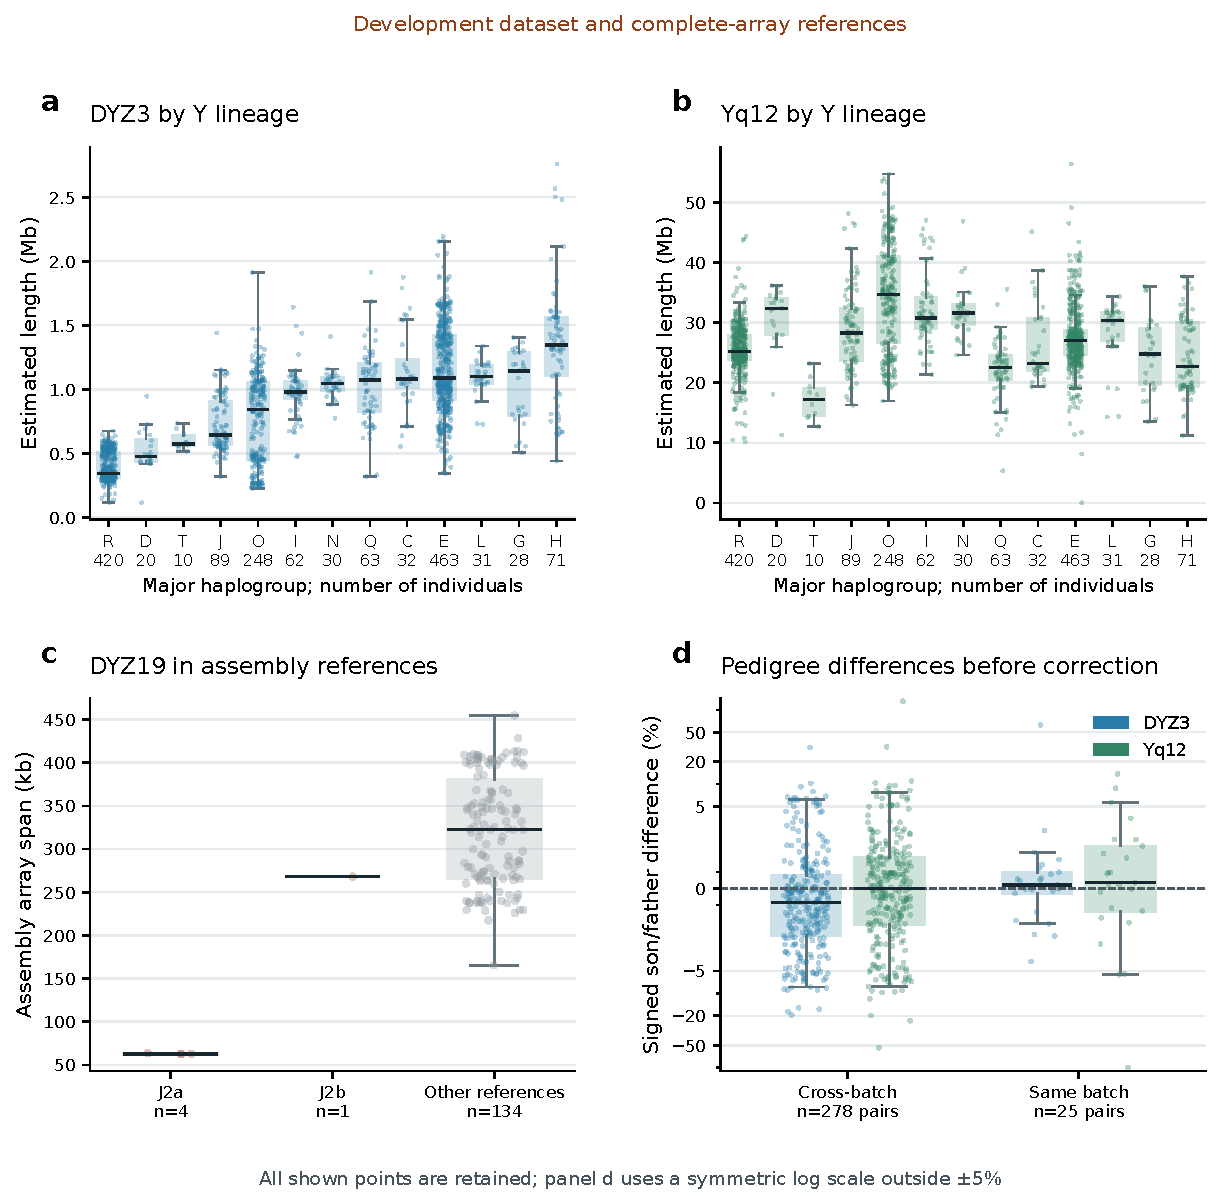
\includegraphics[width=\textwidth]{figures/figureS1_development_checks.pdf}
\caption{\textbf{Supporting development-catalog distributions and pedigree checks.} \textbf{a,b}, DYZ3 and Yq12 estimates by major haplogroup, retaining groups with at least ten individuals. \textbf{c}, DYZ19 spans in all 139 quality-passing assembly references, grouped by the catalog's earlier lineage annotations. \textbf{d}, Signed father--son length differences after requiring dosage $\geq0.9$ in both individuals. Cross-batch pairs have the father in the original batch and the son in the additional batch; same-batch pairs are both in the additional batch. The two reverse cross-batch pairs are omitted. No batch correction is applied. The axis is linear between $-5\%$ and $+5\%$ and logarithmic outside. Boxes show medians and interquartile ranges; whiskers end at the most extreme values within 1.5 interquartile ranges, and points show individual observations. These panels describe the development dataset and its earlier calibration.}\label{fig:development-checks}
\end{figure}
\endgroup

\begingroup
\renewcommand{\thefigure}{S2}
\begin{figure}[tbp]
\centering
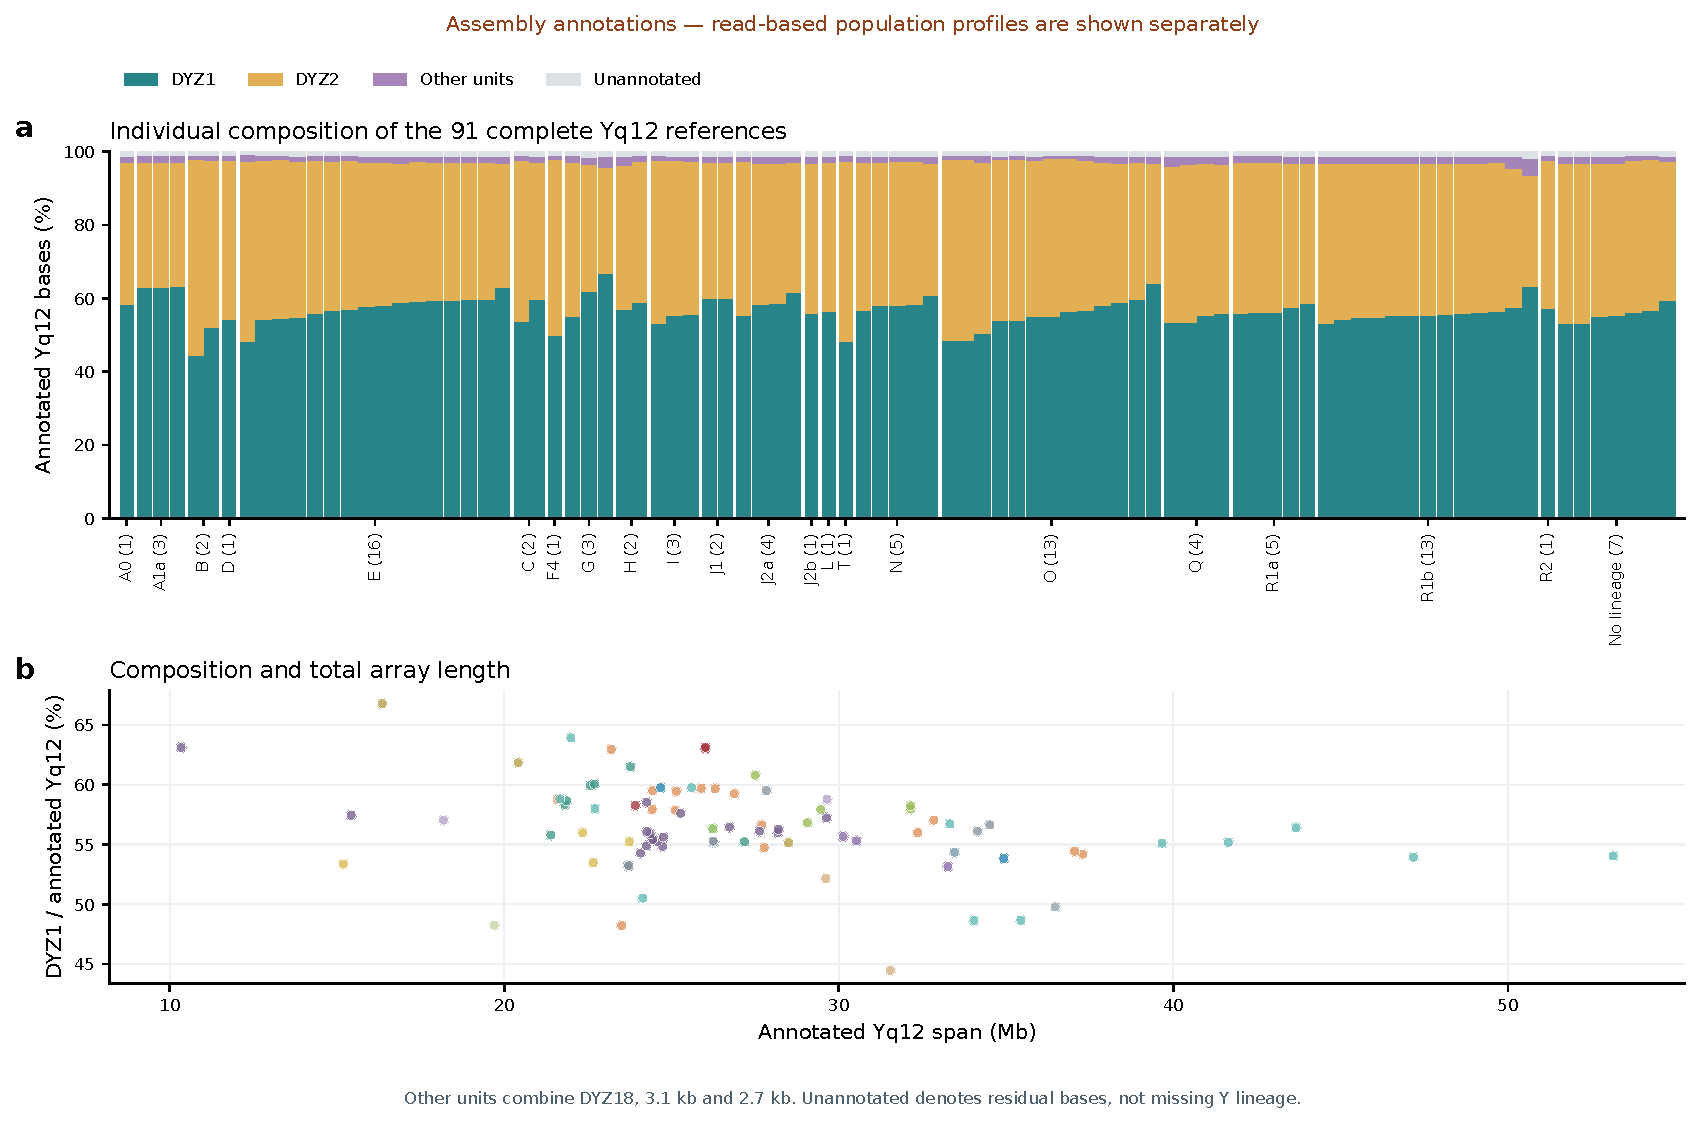
\includegraphics[width=\textwidth]{figures/figureS2_yq12_composition.pdf}
\caption{\textbf{Individual composition of complete Yq12 assembly references.} \textbf{a}, Per-individual composition of all 91 complete reference arrays, grouped by Y clade and sorted by DYZ1 fraction within each clade. Counts below groups give the number of references. The final seven references lack matching lineage metadata. DYZ1, DYZ2, other units (DYZ18, 3.1 kb and 2.7 kb) and residual unannotated bases sum to the annotated Yq12 span. \textbf{b}, DYZ1 fraction against annotated Yq12 span in the same 91 references. Colours denote broad Y lineages as in Fig.~\ref{fig:biology}a; grey marks references without lineage metadata. The plot is descriptive and both axes use the same span. These are assembly annotations; the read-based population estimates are shown separately in Supplementary Fig.~\ref{fig:frozen-population}.}\label{fig:yq12-composition}
\end{figure}
\endgroup

\begingroup
\renewcommand{\thefigure}{S3}
\begin{figure}[tbp]
\centering
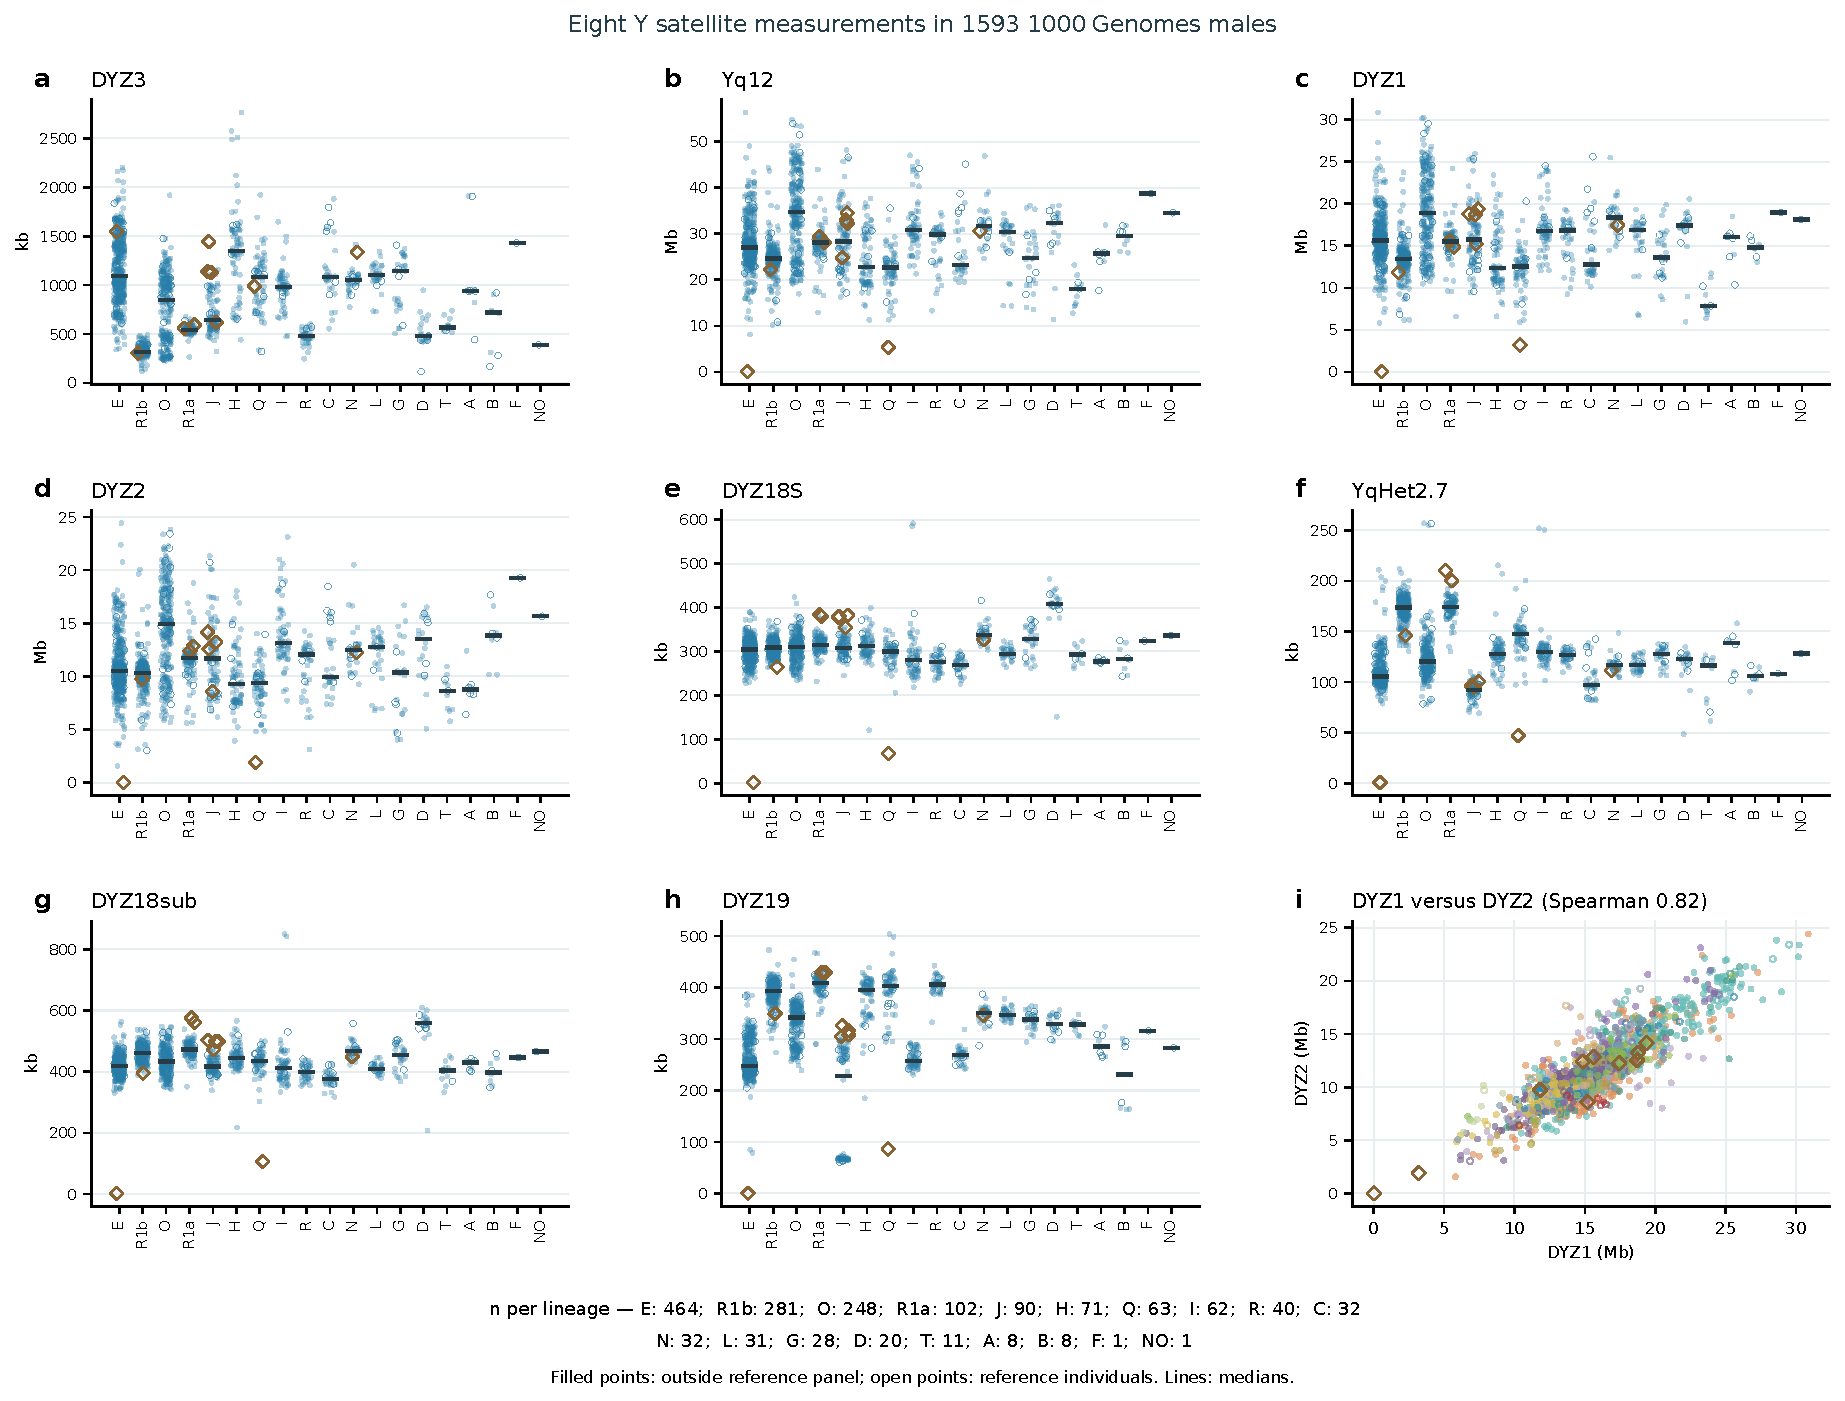
\includegraphics[width=\textwidth]{figures/figureS3_frozen_population.pdf}
\caption{\textbf{Eight satellite measurements across the analysed population.} \textbf{a--h}, Estimated lengths by broad Y lineage for all 1,597 males with estimates, retaining rare groups. Sample counts are listed below the panels; horizontal lines show medians. \textbf{i}, DYZ1 against DYZ2 estimated base-pair lengths, coloured by lineage. Filled circles are outside the calibration panel and open circles are reference individuals. Diamonds identify arm-imbalanced or Yp-depleted profiles, excluded from medians and correlation estimates. Reference estimates can be in-sample. Outputs are calibrated separately and include overlapping targets, so they are not an exact partition of Yq12. Uneven sampling and family dependence limit population-frequency interpretation.}\label{fig:frozen-population}
\end{figure}
\endgroup

\begingroup
\renewcommand{\thefigure}{S4}
\begin{figure}[tbp]
\centering
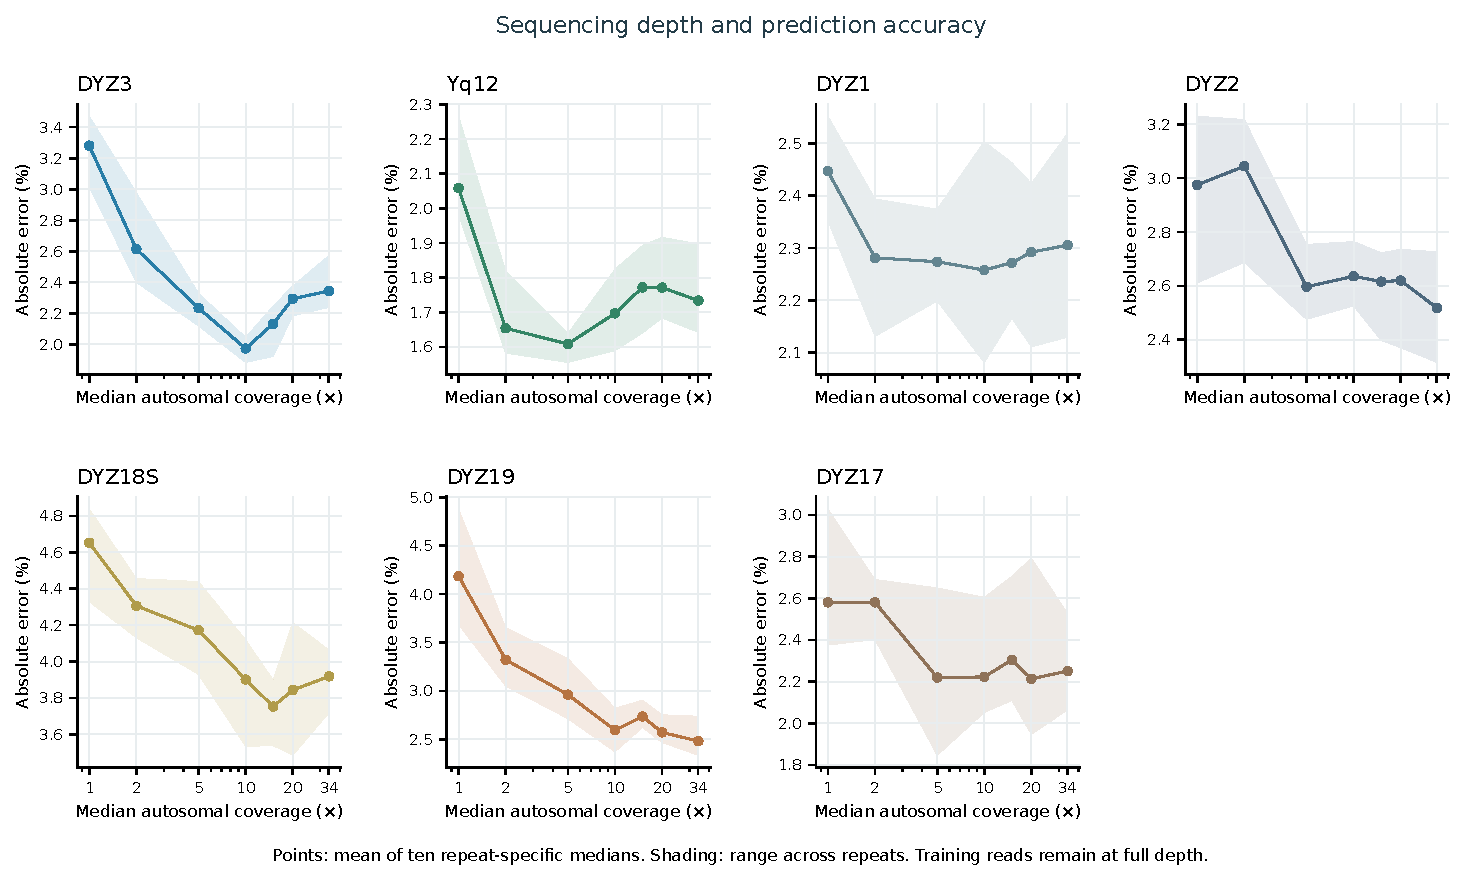
\includegraphics[width=\textwidth]{figures/figureS4_frozen_depth.pdf}
\caption{\textbf{Depth sensitivity of all eight targets and the DYZ1:DYZ2 ratio.} Test reads are thinned to fractions 1, 0.667, 0.5, 0.333, 0.167, 0.067 and 0.033, while training reads retain full depth. The x-axis gives median autosomal depth. Points show the mean of ten grouped-CV repeat-specific median absolute percentage errors, with shading showing their range. These ranges are not confidence intervals. Evaluated counts are 104 for DYZ3, 118 for DYZ19, 81 for Yq12, DYZ2 and the ratio, and 82 for DYZ1, DYZ18S, YqHet2.7 and DYZ18sub. Downsampling reuses the same individuals, and its full-depth baseline matches the ten repeats in Table~\ref{tab:accuracy}.}\label{fig:frozen-depth}
\end{figure}
\endgroup

\begingroup
\renewcommand{\thefigure}{S5}
\begin{figure}[tbp]
\centering
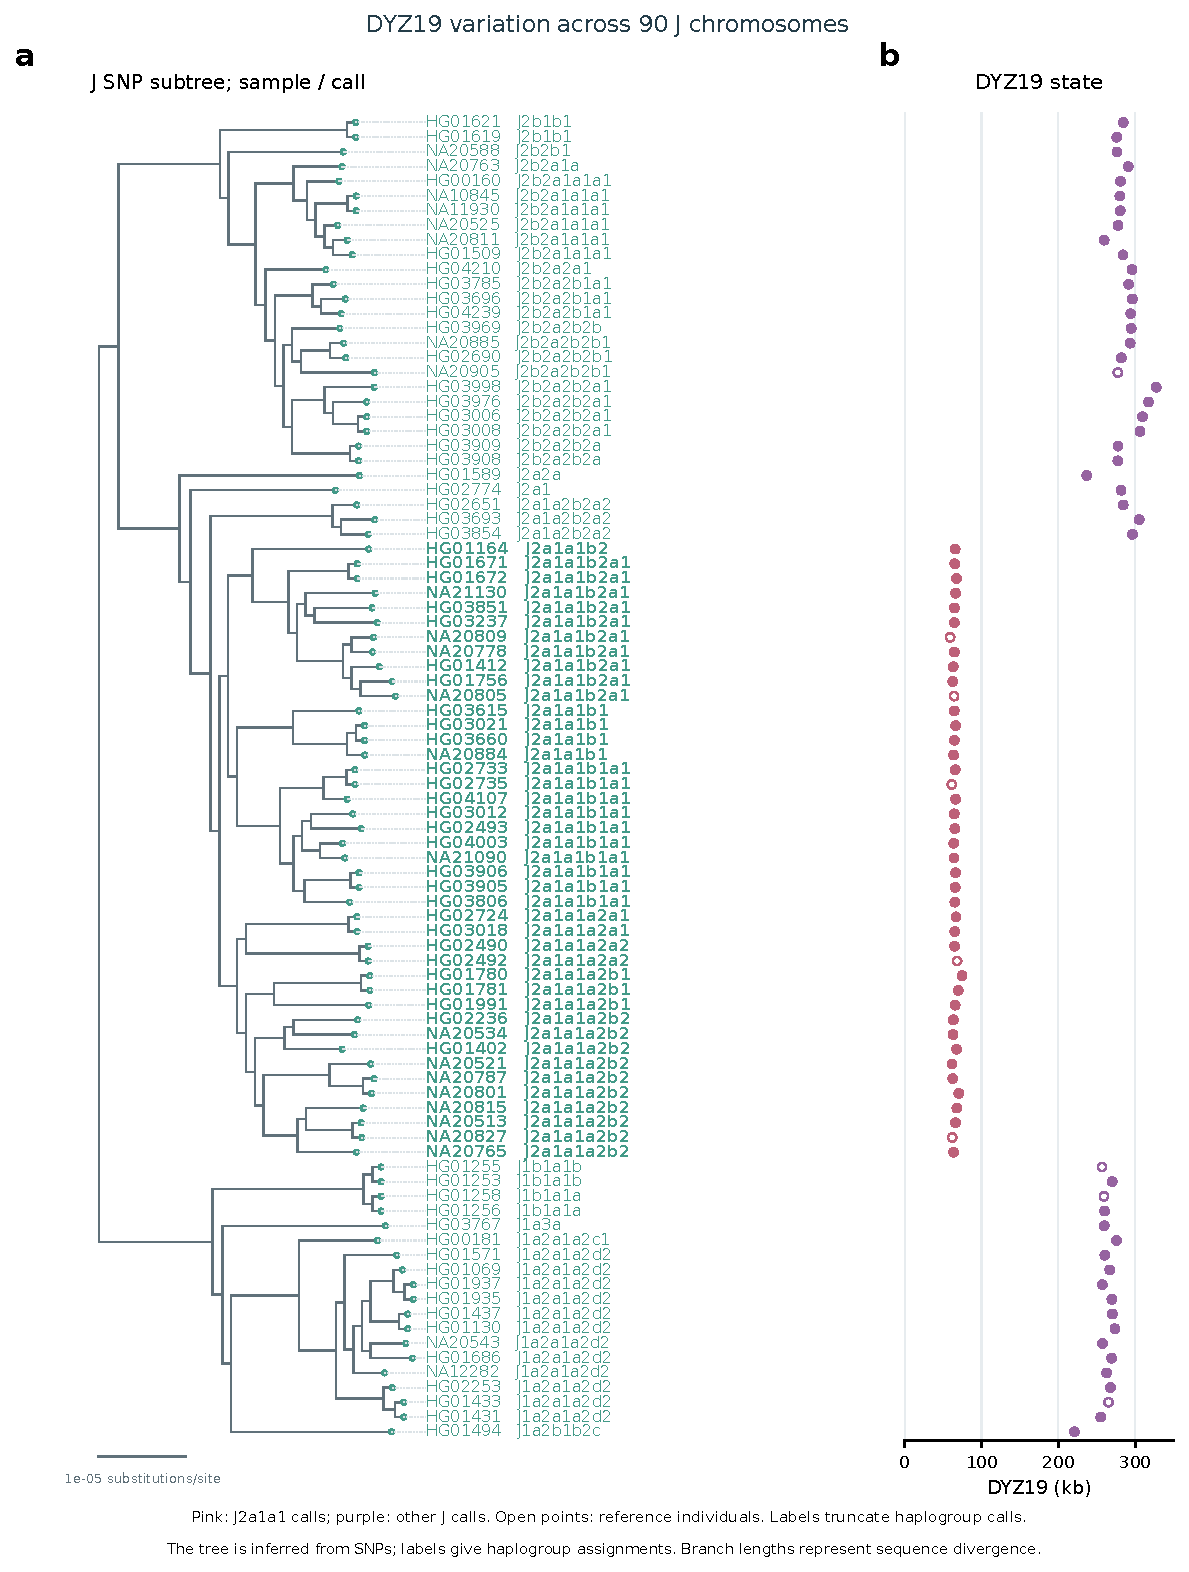
\includegraphics[width=.94\textwidth]{figures/figureS5_J_DYZ19.pdf}
\caption{\textbf{DYZ19 estimates aligned to the provisional SNP tree of all 90 sampled J chromosomes.} \textbf{a}, Pruned tree retaining branch lengths; tips give sample identifiers and abbreviated ISOGG 2019 calls. \textbf{b}, Read-based DYZ19 estimates, with J2a1a1 calls in pink and other J calls in purple; open symbols mark calibration-reference individuals. The short-state groups have distinct J2a1a1a and J2a1a1b calls within a single clade; J2a1a2 lies outside it. The tree is used descriptively; the number and timing of state transitions were not inferred.}\label{fig:j-dyz19}
\end{figure}
\endgroup


\clearpage
\begingroup
\renewcommand{\thefigure}{S6}
\begin{figure}[p]
\centering
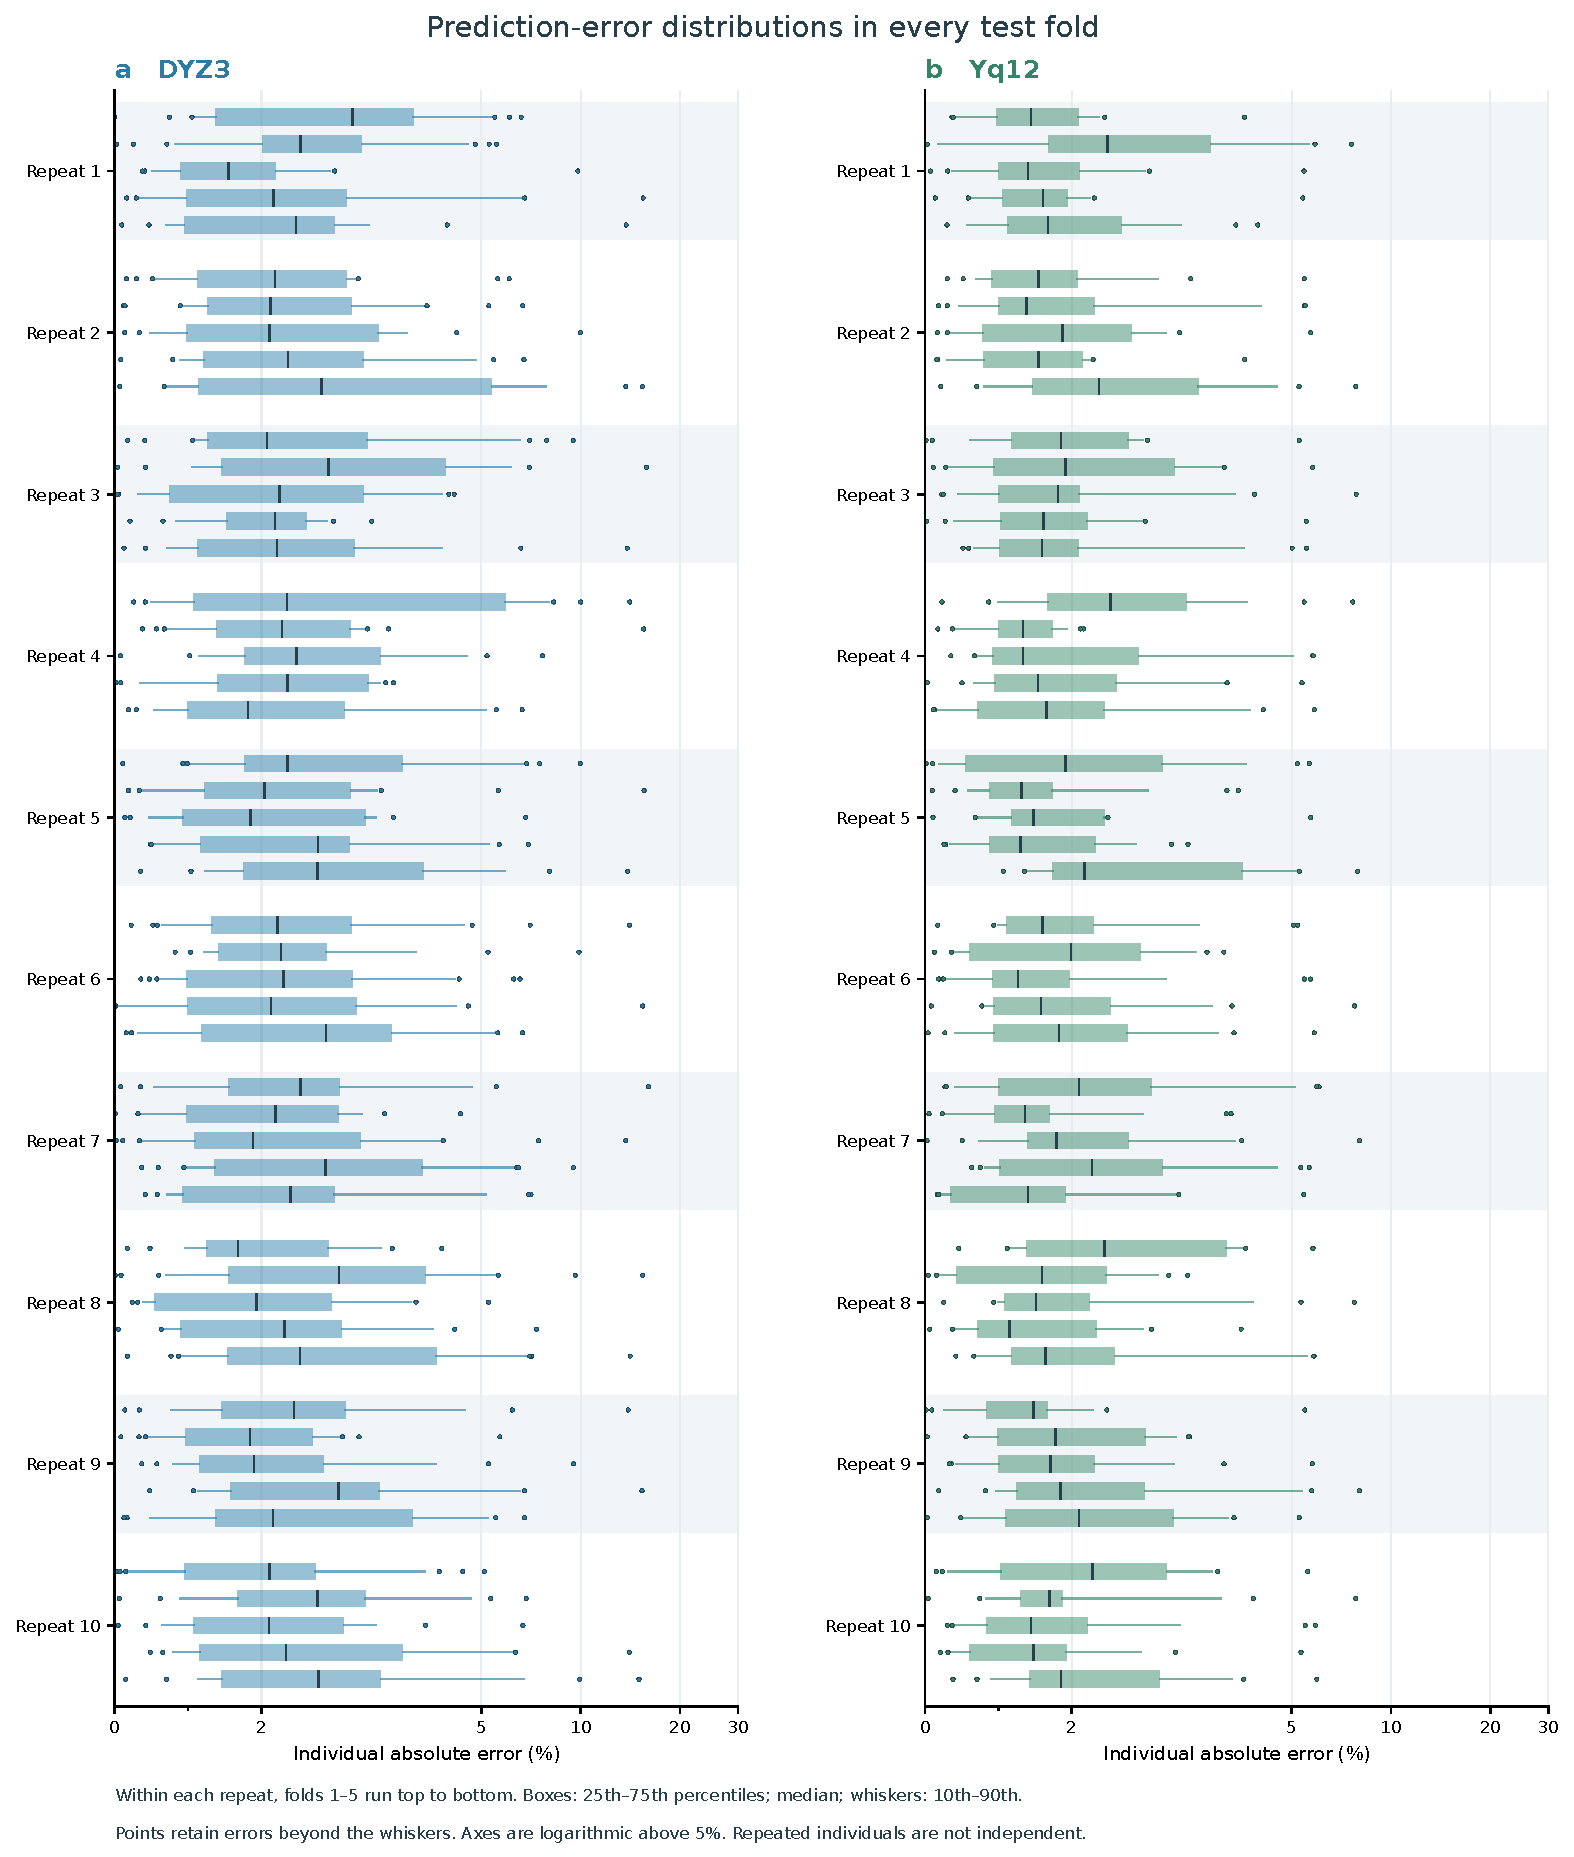
\includegraphics[page=1,width=\textwidth,height=.75\textheight,keepaspectratio]{figures/figureS6_cv_folds.pdf}
\caption{\textbf{Prediction-error variability in every cross-validation fold.} \textbf{a,b}, DYZ3 and Yq12. Each target shows all five test-fold distributions within each of ten repeats, with folds 1--5 running from top to bottom. Boxes span the 25th--75th percentiles, central lines mark medians and whiskers end at the 10th and 90th percentiles; points retain errors beyond the whiskers. Axes are linear through 5\% and logarithmic above. Repeated predictions of the same individual are not independent biological observations.}\label{fig:cv-folds}
\end{figure}
\endgroup

\clearpage
\begingroup
\renewcommand{\thefigure}{S6}
\begin{figure}[p]
\centering
\includegraphics[page=2,width=\textwidth,height=.75\textheight,keepaspectratio]{figures/figureS6_cv_folds.pdf}
\caption{\textbf{Prediction-error variability in every cross-validation fold (continued).} \textbf{c,d}, DYZ1 and DYZ2. Each target shows all five test-fold distributions within each of ten repeats, with folds 1--5 running from top to bottom. Boxes span the 25th--75th percentiles, central lines mark medians and whiskers end at the 10th and 90th percentiles; points retain errors beyond the whiskers. Axes are linear through 5\% and logarithmic above. Repeated predictions of the same individual are not independent biological observations.}
\end{figure}
\endgroup

\clearpage
\begingroup
\renewcommand{\thefigure}{S6}
\begin{figure}[p]
\centering
\includegraphics[page=3,width=\textwidth,height=.75\textheight,keepaspectratio]{figures/figureS6_cv_folds.pdf}
\caption{\textbf{Prediction-error variability in every cross-validation fold (continued).} \textbf{e,f}, DYZ18S and YqHet2.7. Each target shows all five test-fold distributions within each of ten repeats, with folds 1--5 running from top to bottom. Boxes span the 25th--75th percentiles, central lines mark medians and whiskers end at the 10th and 90th percentiles; points retain errors beyond the whiskers. Axes are linear through 5\% and logarithmic above. Repeated predictions of the same individual are not independent biological observations.}
\end{figure}
\endgroup

\clearpage
\begingroup
\renewcommand{\thefigure}{S6}
\begin{figure}[p]
\centering
\includegraphics[page=4,width=\textwidth,height=.75\textheight,keepaspectratio]{figures/figureS6_cv_folds.pdf}
\caption{\textbf{Prediction-error variability in every cross-validation fold (continued).} \textbf{g,h}, DYZ18sub and DYZ19. Each target shows all five test-fold distributions within each of ten repeats, with folds 1--5 running from top to bottom. Boxes span the 25th--75th percentiles, central lines mark medians and whiskers end at the 10th and 90th percentiles; points retain errors beyond the whiskers. Axes are linear through 5\% and logarithmic above. Repeated predictions of the same individual are not independent biological observations.}
\end{figure}
\endgroup


\clearpage

\clearpage
\begingroup
\renewcommand{\thefigure}{S6}
\begin{figure}[p]
\centering
\includegraphics[page=5,width=\textwidth,height=.75\textheight,keepaspectratio]{figures/figureS6_cv_folds.pdf}
\caption{\textbf{Prediction-error variability in every cross-validation fold (continued).} \textbf{i}, Derived DYZ1:DYZ2 ratio. Each error pairs component predictions from the same individual, repeat and fold. All five test folds within each of ten repeats are shown; boxes, points and axes follow the preceding pages.}
\end{figure}
\endgroup
\clearpage

\begingroup
\renewcommand{\thefigure}{S7}
\begin{figure}[p]
\centering
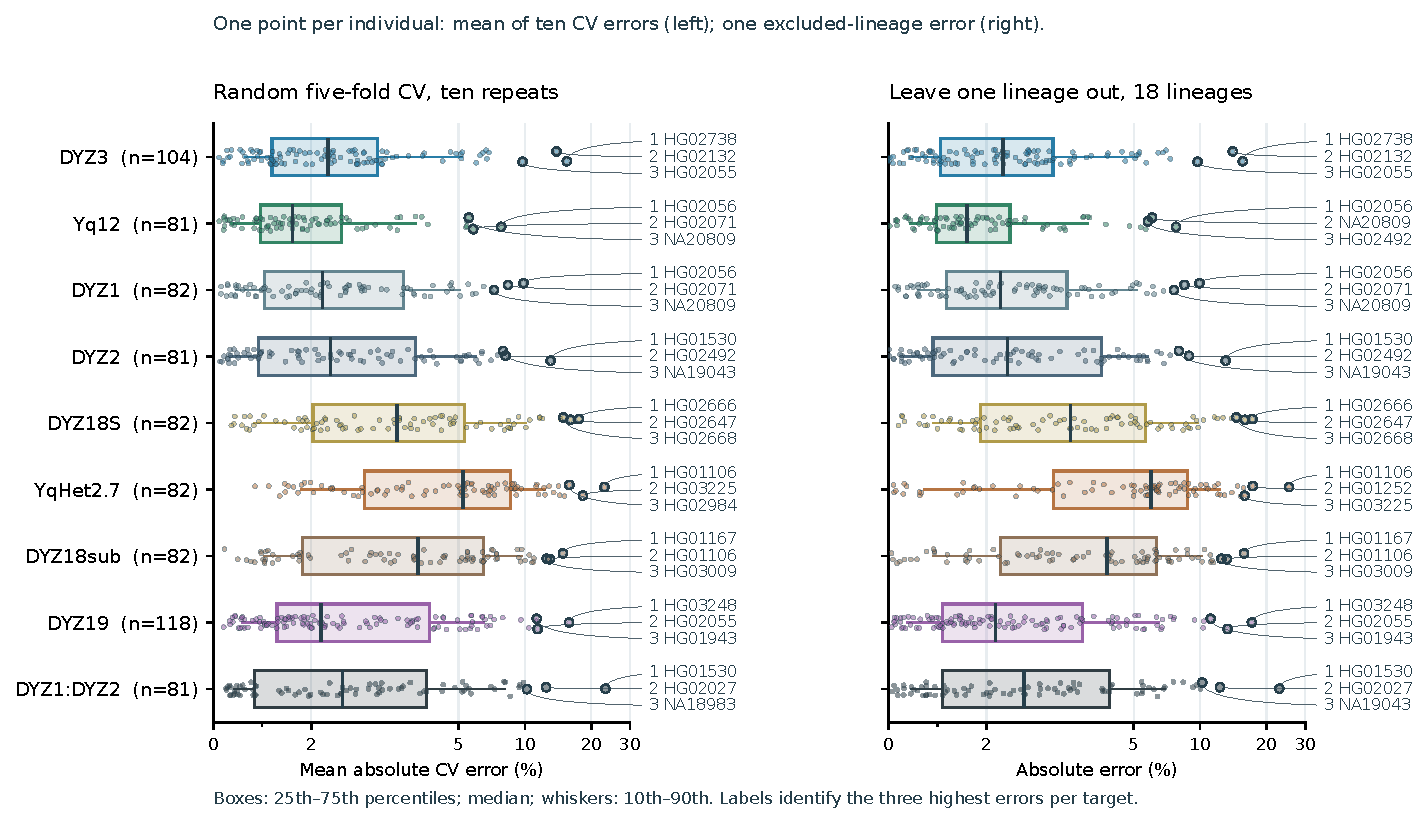
\includegraphics[width=\textwidth]{figures/figureS7_lineage_validation.pdf}
\caption{\textbf{Random cross-validation and exclusion of entire Y lineages.} Left: each point averages an individual's ten absolute percentage errors from family-grouped random five-fold CV. Right: each point is the individual's single absolute percentage error when its entire lineage is excluded from training, pooling all 18 excluded-lineage tests. Training also excludes any recorded family shared with test individuals. Each measurement has the same evaluated individuals in both panels; the final row is the derived DYZ1:DYZ2 ratio. Boxes span the 25th--75th percentiles, central lines mark medians and whiskers end at the 10th and 90th percentiles. All individual points are shown; labels identify the three largest displayed errors per target. Axes are linear through 5\% and logarithmic above.}\label{fig:lineage-validation}
\end{figure}
\endgroup
\clearpage


\clearpage
\begingroup
\renewcommand{\thefigure}{S8}
\begin{figure}[p]
\centering
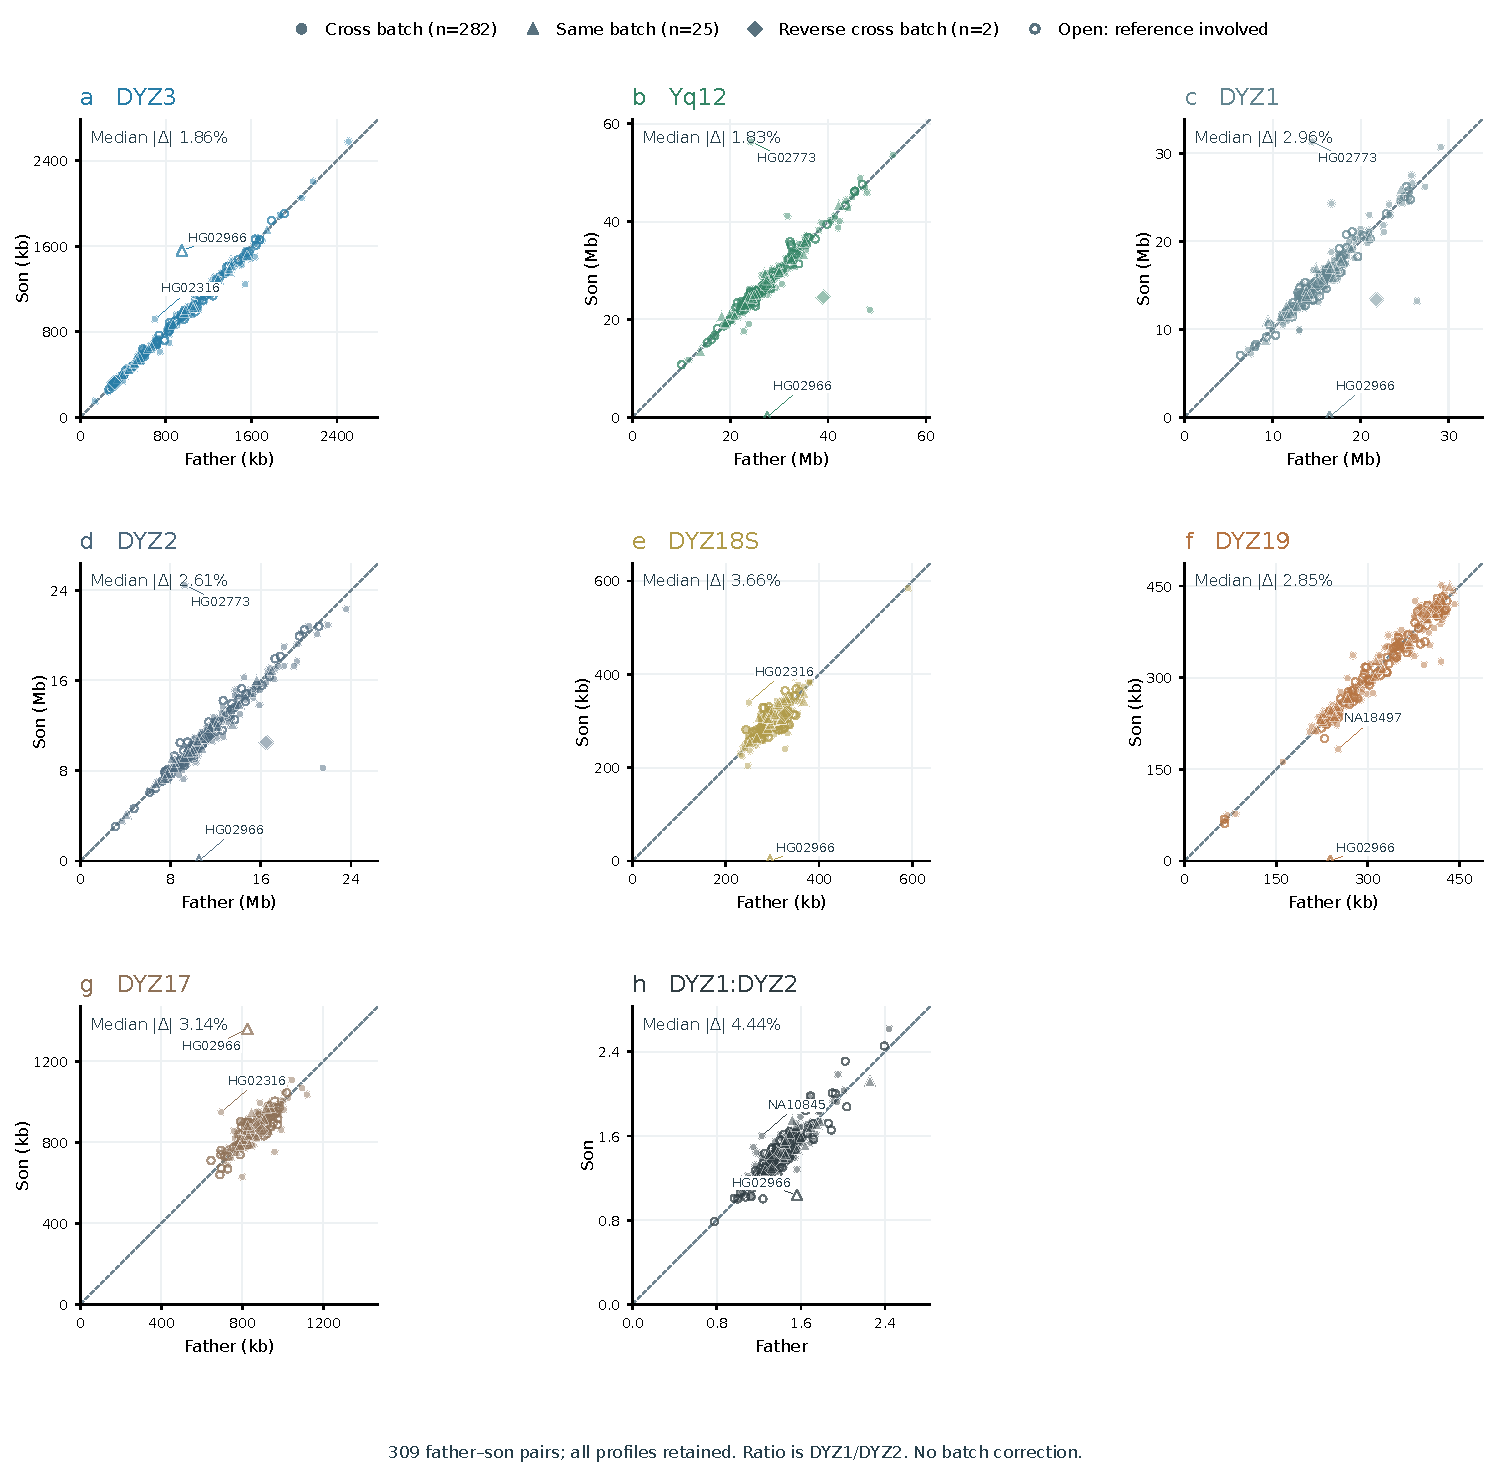
\includegraphics[page=1,width=\textwidth,height=.75\textheight,keepaspectratio]{figures/figureS8_all_pedigrees.pdf}
\caption{\textbf{Father--son concordance for every satellite target and the DYZ1:DYZ2 length ratio.} \textbf{a--i}, All 309 pairs with complete estimates, shown for the eight targets and the derived ratio. Each point compares the father's and son's estimates; diagonals mark equality and axes have matching limits. Colours match Fig.~\ref{fig:method}b. Shapes distinguish the 282 original-father/additional-son pairs, 25 same-batch pairs and two reverse cross-batch pairs. Open points identify 78 pairs involving a calibration-reference individual. Annotations give median absolute son/father differences; labels identify sons in the two pairs with the largest absolute percentage differences when these exceed 10\%. All complete profiles, including arm-imbalanced or Yp-depleted profiles, remain visible. No dosage cutoff or batch correction is applied. Targets use their indicated length units; the ratio is dimensionless. Pedigree pairs can share relatives and are not independent observations.}\label{fig:all-pedigrees}
\end{figure}
\endgroup

\clearpage
\begingroup
\renewcommand{\thefigure}{S8}
\begin{figure}[p]
\centering
\includegraphics[page=2,width=\textwidth,height=.75\textheight,keepaspectratio]{figures/figureS8_all_pedigrees.pdf}
\caption{\textbf{Father--son concordance for every satellite target and the DYZ1:DYZ2 length ratio (continued).} \textbf{a--i}, Signed differences $100(\widehat L_{\mathrm{son}}/\widehat L_{\mathrm{father}}-1)$ for the same measurements and pairs. For the ratio, $\widehat L$ denotes the individual's DYZ1:DYZ2 ratio. Batch contrasts are shown separately, including the two reverse-direction pairs. Points show every pair; horizontal segments span the 25th--75th percentiles, central marks and labels give medians. Difference axes are linear within $\pm5\%$ and logarithmic outside; their ranges retain all observations. Reference-involved pairs remain open. These differences combine technical variation, possible biological changes and flagged structural profiles; they are not mutation-rate estimates.}
\end{figure}
\endgroup
\clearpage

\backmatter

\ifdraftnotes
\bmhead{Acknowledgements}
\draftnote{Add acknowledgements for the source data resources, collaborators and funding after the final analysis scope is fixed.}

\section*{Declarations}

\bmhead{Authors' contributions}
\draftnote{Specify the contributions of Alejandro Ortigas-Vasquez and Andrea Guarracino.}

\bmhead{Competing interests}
\draftnote{Obtain the authors' declarations.}

\fi

\bmhead{Data availability}
We used public 1000 Genomes sequencing data \cite{ByrskaBishop2022}, Y chromosome assemblies \cite{Hallast2026}, HPRC release 2 assemblies \cite{HPRCRelease2} and pedigree sequencing resources \cite{Porubsky2025}. Public KING reports and corrected sample metadata are available from \url{https://www.cog-genomics.org/plink/2.0/resources}. Study data comprise per-sample satellite estimates, reference-array annotations, model parameters, cross-validation predictions, the SNP tree, relatedness tables and geographic metadata.
\draftnote{Insert the archival accession for study-generated data and the source accession/checksum manifest before submission.}

\bmhead{Code availability}
The yruler repository is \url{https://github.com/guarracinolab/yruler}. Analysis code generates the figures and tables from per-sample estimates, validation predictions and source metadata.
\draftnote{Confirm public accessibility, the software licence, a versioned release and an archival identifier before submission. Add the analysis-code release and the commands needed to reproduce the figures and tables.}

\bibliography{refs}

\end{document}
